%==============================================================================
% (c) David Molnar 2015
%==============================================================================

\chapter{Úvod}
Vyvíjet software v dnešní době není jednoduché. Konkurence na trzích je silná, požadavky na software se mění velice rychle a často je potřeba vydávat novou verzi aplikace co nejrychleji.

Za základní zásadu pro vývojový tým můžeme považovat Continuous Integration. Pomocí tohoto konceptu zůstane tým v synchronizaci a dokáže odstranit zpoždění způsobené integračními chybami. Je důležité si ale uvědomit, že Continous Integration je pouze prvním krokem k dosažení cíle. Další stanice je Continuous Delivery, tzn. nejenom častá integrace, ale i časté nasazení a uvolnění nové verze aplikace do produkce. Rozchodit nasazení ve smyslu Continuous Delivery není jednoduché, záleží to samozřejmě i na složitosti projektu. Nesmíme se ale zapomenout na okamžité výhody. Dlouhé, pracné a problematické vydávání verzí a jejich nasazení se stane věcí minulosti. Díky tomu zákazníci uvidí okamžitý pokrok vývoje objednaného produktu, který dodá funkcionalitu, kterou potřebují a využívají každý den. Je potřeba se zmínit i o výhodě, že tím se také odstraní jeden z největších zdrojů stresu a napětí v týmu.

Velice inspirativní je projekt a tým vedený panem Kentem Beckem \cite{ContDelivery}. Tento velice disciplinovaný tým každý večer nasazoval novou verzi své aplikace přímo do produkce. Takový způsob implementace má několik výhod: napsaný a hotový kód neleží ve verzovacím systému\footnote{SVN, Git, TFS atd.} bez využití a tým dokáže velice rychle reagovat na problémy a na nové příležitosti. Navíc je zajímavý, že tento způsob práce vedl k prohloubení vztahů mezi členy týmu a nárůstu důvěry zákazníka ve firmě. 

Continuous Delivery dokáže snížit dobu trvání cyklu, od první myšlenky a nápadu až do použitelný software. Myšlení ve smyslu Continuous Delivery upadlo na dlouhou dobu v zapomenutí, někde mezi vývojovým a nasazovacím týmem. Proto je velice důležité tyto dva týmy co nejvíce spojit. Nesmíme se zapomenout na to, že základem všeho je vysoká stupeň automatizace -- jednotlivá operace budou rychlé, opakovatelné, snadno testovatelné a kvalitní (bez chyb).

Našimi hlavními průvodci v této práci budou Jez Humble a David Farley, průkopníci a známí aktivisti zásad Continous Delivery. Jejich kniha \cite{ContDelivery} bude pro nás sloužit jako Bible. 

Tato práce se detailně zabývá implementací zásad Continuous Delivery při urychlení vývoje a nasazení jedné ukázkové aplikace. Ukázkový projekt je webová aplikace s relační databází MSSQL. Obsahuje i další části, které budou popsané v kapitole \ref{ch:impl}. 

V kapitole \ref{ch:teorie} bude čtenář obeznámen se základními pojmy z oblasti agilních metodik vývoje a doručení softwarových produktů. Kapitola \ref{ch:impl} se detailně zabývá návrhem a implementací ukázkové aplikace. Vzhledem k tomu, že je to ukázková aplikace, nebudou všechny detaily implementovány. V pokračování je popsán vývoj jednotlivých nástrojů a vytvoření infrastruktury (testovací prostředí, skripty, konfigurace atd.), kam bude aplikace nasazena. Vyhodnocení výsledků se uskuteční v kapitole \ref{ch:vyslekdy}. Pokusíme se porovnat výhody a nevýhody zásad Continous Delivery. V závěru v kapitole \ref{ch:zaver} bude následovat souhrn práce.

Naším cílem bude tedy ukázat, že je možný dodat vysoce kvalitní softwarový produkt velice často, třeba i denně a to bez zbytečných problémů a zádrhelů. Budeme k tomu používat hlavně Microsoft technologie.

V celé této práci budeme označovat pojmy Continous Delivery zkratkou CD a Continous Integration zkratkou CI. Ostatní zkratky jsou popsány v sekci \ref{pojmy}. V oblasti CD existuje mnoho nových pojmů, které ale nebyly zatím přeloženy do českého jazyka. Abychom předešli zbytečných nejasností, tyto pojmy budeme používat v původní podobě, tedy angličtině.

\chapter{Teoretická část}
\label{ch:teorie}
V této kapitole seznámíme čtenáře se základy Continous Delivery. Ukážeme, jaké problémy lze vyřešit pomocí tohoto konceptu. Čerpáme hlavně z knihy\cite{ContDelivery}.

\section{Deployment pipeline}
Ve vývoji software je velice důležitý, jakým způsobem bude vyvíjený produkt dodán uživateli. Jaká je rychlost, efektivita, spolehlivost a kvalita dodání. Většina vývojářů se soustředí na analýzu, psaní kódu a někteří i na testování (jednotkové testy, integrační testy atd.).
Existuje spousta metodik pro vývoj software, většina z nich se ale  soustřeďuje na zpracování požadavku a na jeho vliv na proces vývoje.

Nejdůležitější technikou pro nás bude tzv. deployment pipeline. Deployment pipeline je automatizovaná implementace procesu sestavení (build), testování a nasazení naší aplikace. Samozřejmě každá organizace bude mít svoji vlastní implementaci, nicméně principy a zásady budou stejné. Na obrázku \ref{fig:pipeline_overview} je vidět základní, jednoduchý postup kroků probíhajících v rámci deployment pipeline. Další obrázek, \ref{fig:pipeline}, ukazuje kompletní příklad, kde je vidět i verzovací systém a jednotlivá fáze pracovního postupu.

\begin{figure}[]
  \centering
  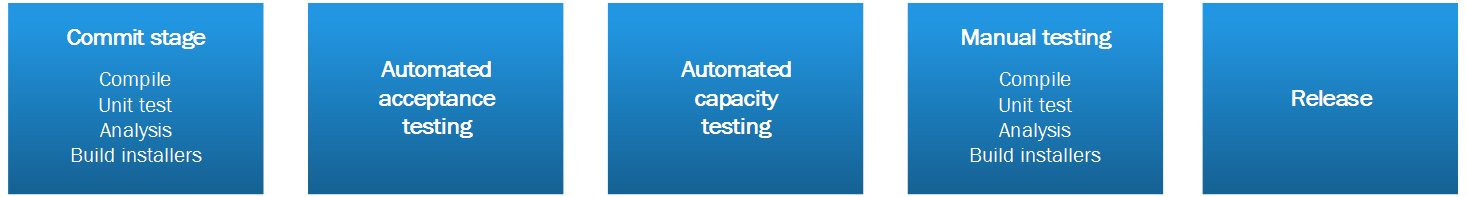
\includegraphics[width=15cm]{fig/pipeline_overview.png}
  \caption{Kroky probíhající v rámci deployment pipeline (přezvato z \cite{ContDelivery})}
  \label{fig:pipeline_overview}
\end{figure}

\begin{figure}[]
  \centering
  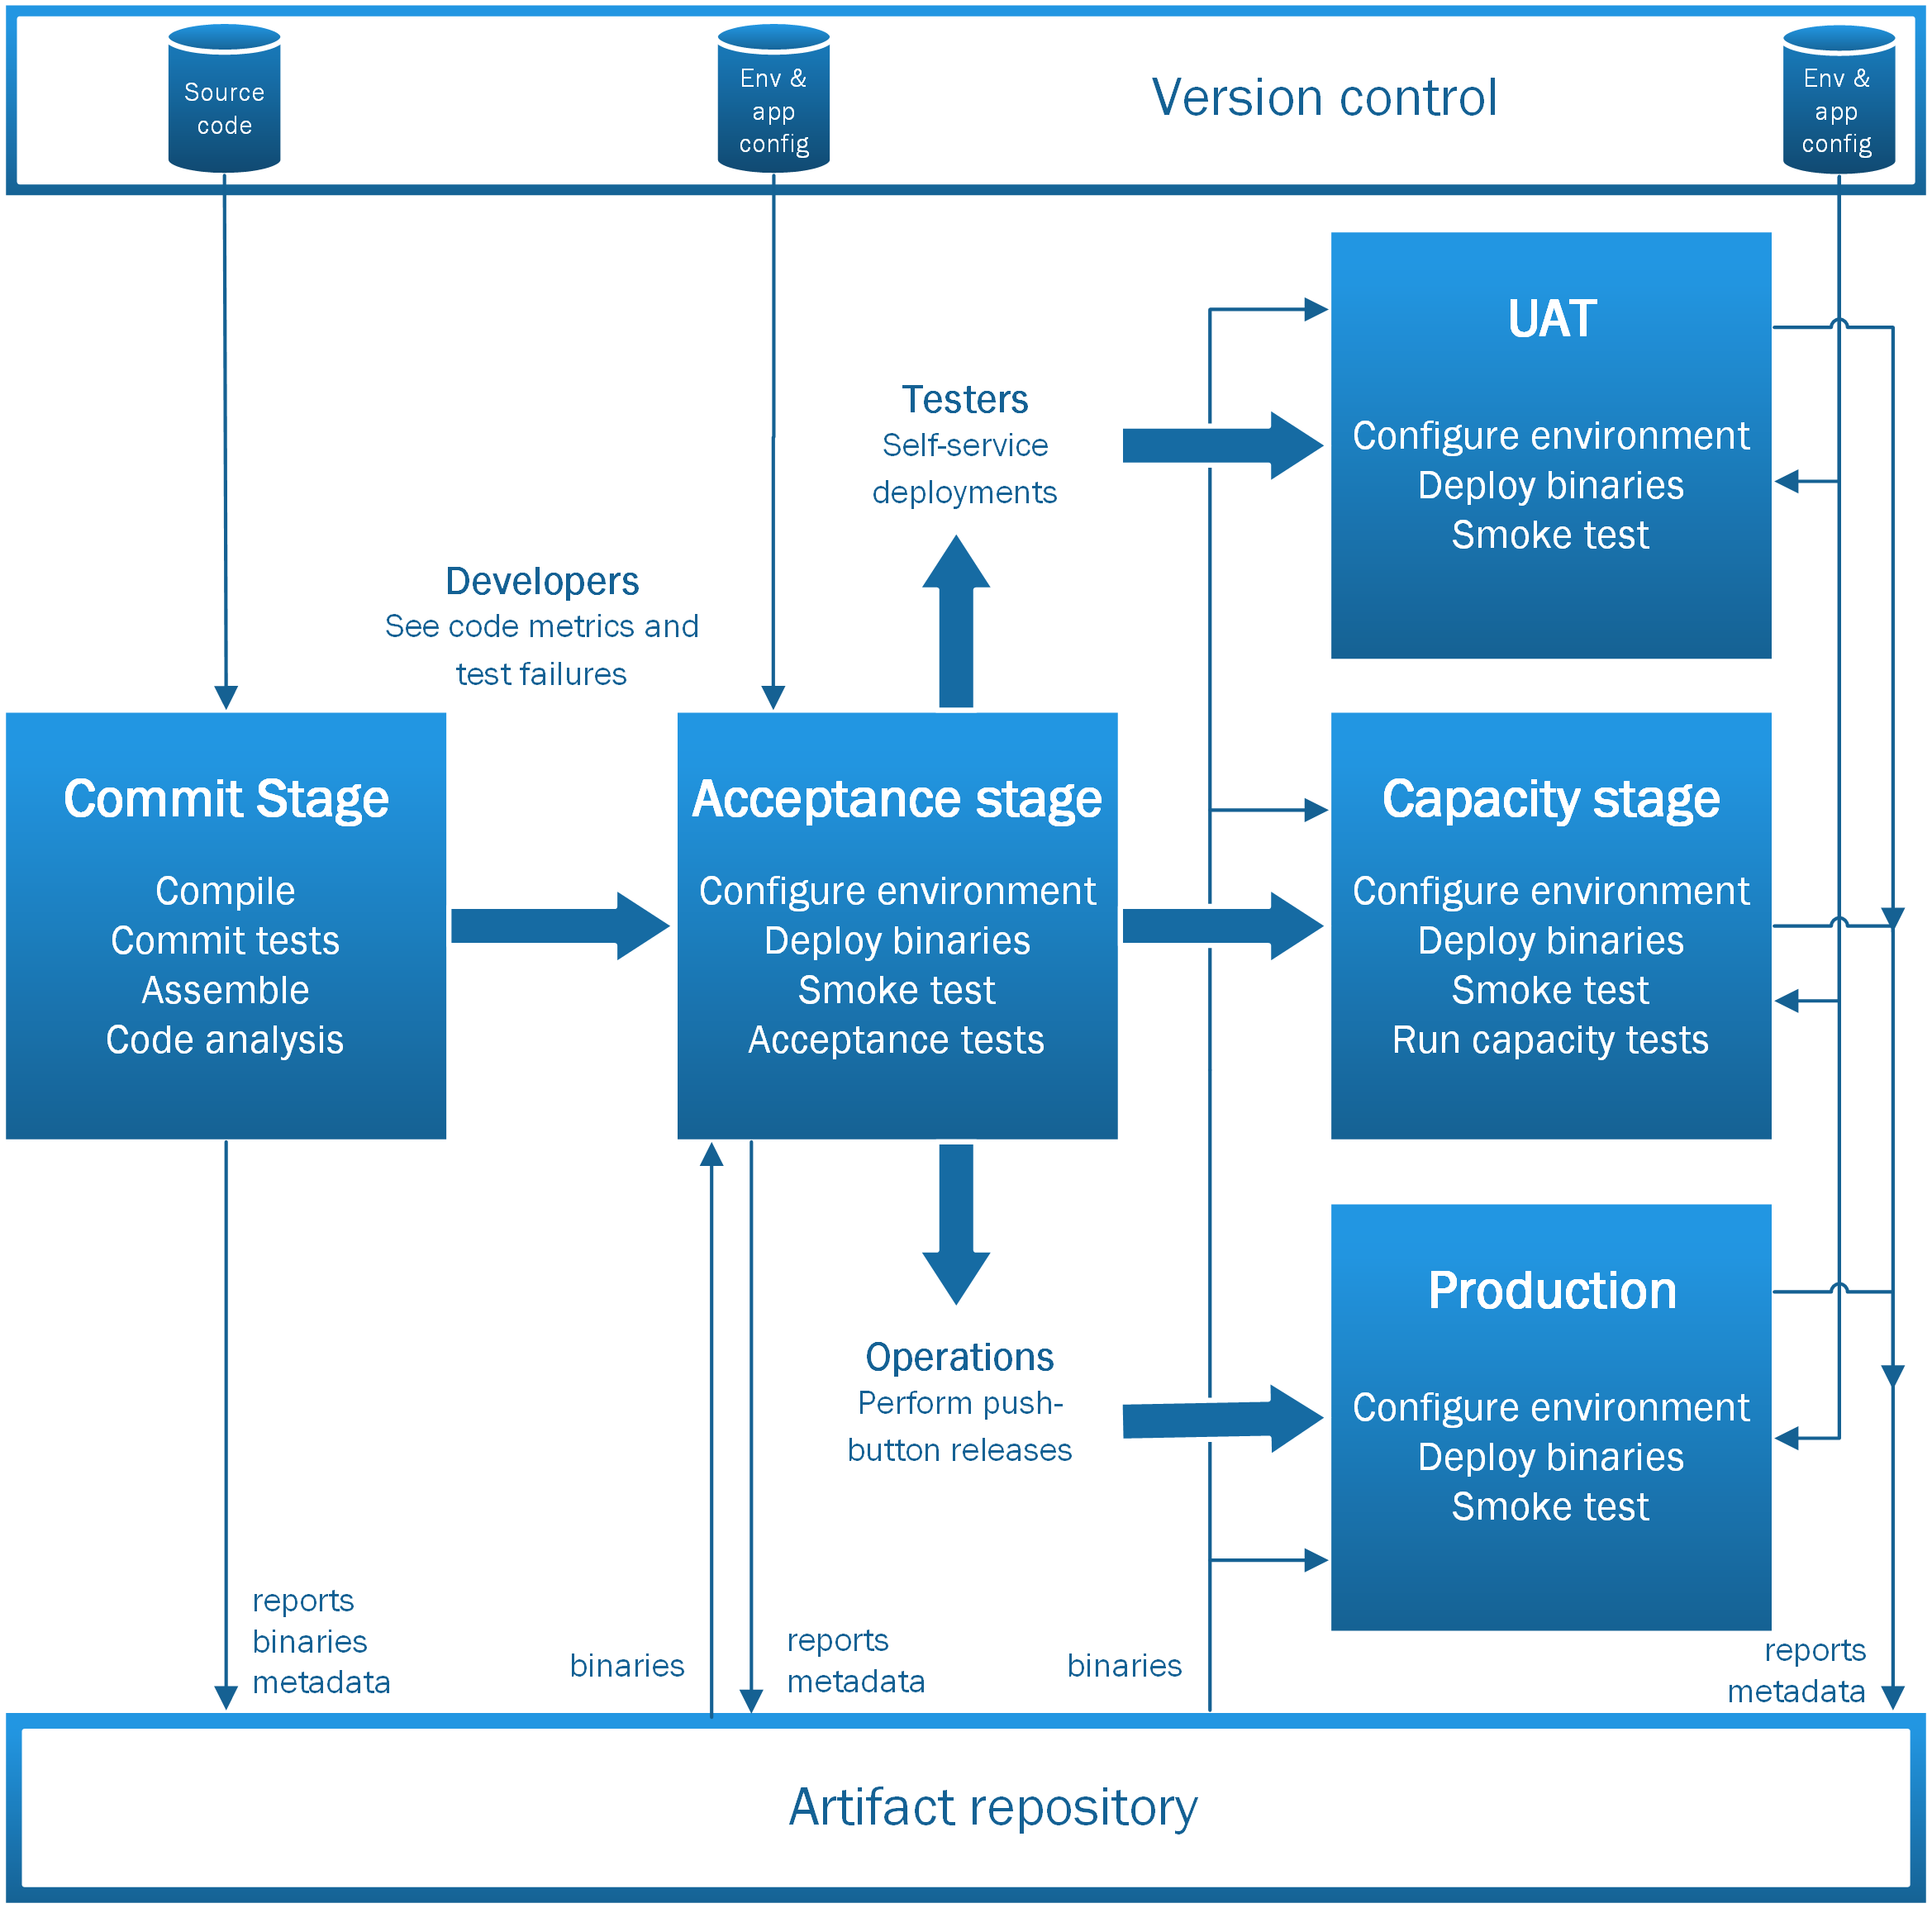
\includegraphics[height=12cm]{fig/pipeline_basic.png}
  \caption{Jednotlivé části a fáze v deployment pipeline (přezvato z \cite{ContDelivery})}
  \label{fig:pipeline}
\end{figure}

Každá změna ve zdrojovém kódu, v konfiguraci nebo v prostředí způsobuje vytvoření nové instance pipeline-u (viz obrázek \ref{fig:pipeline_commit}). První krok je vytvoření binárek a installerů. Pak následuje testování, které ověří, jestli produkt má dostatečnou kvalitu. Každý test nám poskytne důvěru, že daná kombinace binárek, konfigurace a prostředí bude fungovat. Testování nemusí být vždy plně automatizované -- často je potřeba, aby člověk ověřoval výstupy manuálně. 

\begin{figure}[]
  \centering
  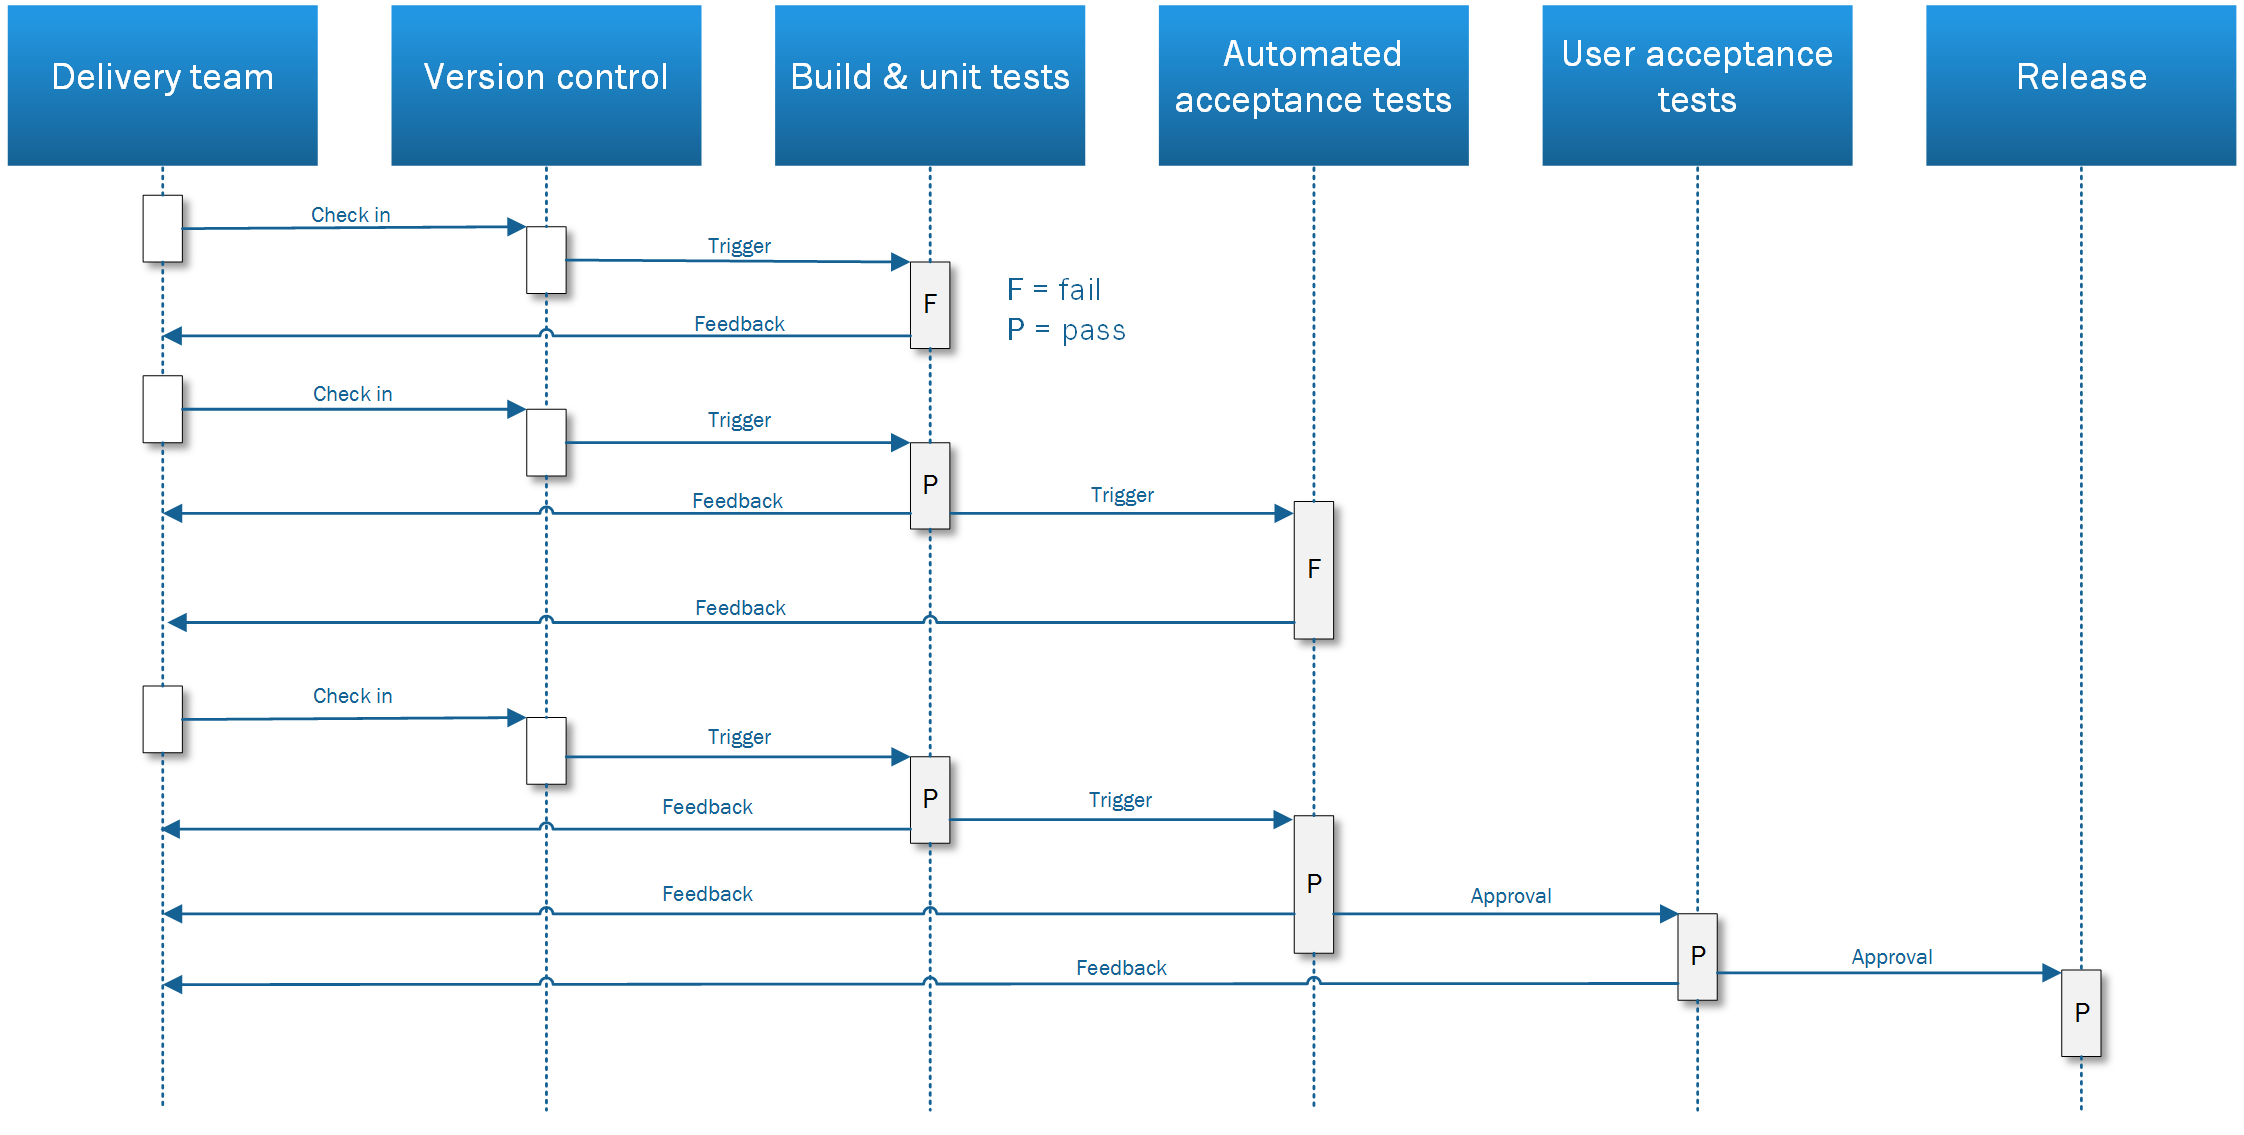
\includegraphics[width=15cm]{fig/pipeline_changes.png}
  \caption{Změny přecházející se přes deployment pipeline (přezvato z \cite{ContDelivery})}
  \label{fig:pipeline_commit}
\end{figure}

Největší výhodou deployment pipeline-u je, že zviditelní každou část vývojového procesu pro všechny členové týmu. Tým takto dokáže zajistit lepší kolaboraci. Další výhodou je i zlepšení zpětné vazby -- problémy jsou identifikovány a odstraněny co nejrychleji. Umožňuje i to, aby tým mohl nasazovat jakoukoli verzi softwaru kdykoli pomocí zcela automatizovaného procesu.

\section{Běžné antipatterny nasazování}
Krok nasazení u většiny moderních aplikací je procesem komplexním, zahrnujícím spoustu dílčích kroků. Mnoho organizací nasazuje software manuálně. Každý krok se provede manuálně, jako atomická operace. Všechna rozhodnutí, dělaná během nasazení, jsou náchylná k lidským chybám. Navíc jednotlivé kroky je možné udělat po každém trošku jinak, co může vést k různým nejasným a nekvalitním výsledkům.

\subsection{Manuální nasazování}
Tento bod může být charakterizován následovně:

\begin{itemize}
  \item Existuje velice detailní dokumentace, který popisuje proces nasazení
  \item Při ověření kvality se spoléhá především na manuální testování 
  \item Příliš časté dotazy na vývojový tým, ohledně vysvětlení chyb při nasazení
  \item Nasazovací proces se v průběhu vydání verze často modifikuje a opravuje
  \item Prostředí mají rozdílná konfigurace, např. aplikační servery s různými konfiguracemi aplikačního poolů, nekonzistentní struktury složek, různá verze prerekvizit atd.
  \item Nasazení a vydání verze trvá hodiny, občas i několik dnů
\end{itemize}

\subsection{Nasazení do produkce až po dokončení vývoje}
V tomto případě je aplikace nasazena do produkce až ve chvíli, kdy vývojový tým zcela dokončil vývoj. Charakterizace:

\begin{itemize}
  \item Jestliže aplikace byla testována, testeři testovali na vývojových stanicích
  \item Lidi z nasazovacího týmu uvidí novou verzi aplikace teprve během nasazení. V některých organizacích existují dva týmy: jeden pro nasazení do testovacího prostředí a jeden pro produkci. Vybudovat prostředí, které je podobné produkci, je velice drahé; přístup k němu je přísně kontrolován, případně je možné, že vůbec neexistuje.
  \item Vývojový tým sestaví binárky, instalátory, konfigurační soubory, databázové migrační skripty a nasazovací dokumentaci, které pak předá nasazovacímu týmu. Tento tým následně provede samotné nasazení -- většinou do prostředí, které předtím nebylo nikdy otestováno.  
  \item Kolaborace mezi vývojovými a nasazovacími týmy je slabé, nebo vůbec neexistuje. Lidé nechtějí zlepšit komunikaci, raději se spoléhají na dokumentaci atd.
\end{itemize}

Slabá spolupráce je pak kompenzována ad-hoc řešením: emaily, telefonní hovory, rychlé opravy. Přináší to stres, spěch a nízkou kvalitu. Disciplinovaný tým zahrne všechny informace o nasazení do nasazovacího plánu, ale i přesto je tento postup málokdy účinný. Většinou je potřeba dodat produkt v určitém termínu, což může vést k nárůstu tlaku mezi členy týmu a ke zhroucení předem definovaného postupu nasazení. 

V následujících kapitolách ukážeme, jak nám může pomoct integrování testovacích a nasazovacích činností do vývojového procesu. Budou to činnosti každodenní práce. Když přijde čas nasazení do produkce, riziko, že něco nefunguje, bude velice malé -- postupy již budou mnohokrát ověřeny a vyzkoušeny týmem v nejrůznějších prostředích. K tomu ovšem musí být zajištěna časná spolupráce všech lidí, podílejících se na vývoji a doručení.

\subsection{Manuální správa konfigurace produktivního prostředí}
Mnoho organizací spravuje konfigurace produktivních prostředí prostřednictvím speciálního týmu -- tzv. nasazovacího týmu. Pokud je potřeba udělat nějakou změnu, např. upravit parametry databázového připojení, zvýšit maximální povolenou velikost příchozí žádosti na webovém serveru, pak potřebné akce provede tento tým zcela manuálně, přímo v produkci. Ve většině případů historie změn neexistuje, pokud ale ano, je to manuální záznam v databázi, na kterou se často zapomene.

\begin{itemize}
  \item Nasazení do testovacího prostředí bylo několikrát úspěšné, nasazení do produkce se přesto nezdaří.
  \item Nasazovací tým dlouhou dobu připravuje prostředí pro nasazení.
  \item Nelze udělat krok zpátky na dřívější konfiguraci systémů, mezi které patří operační systémy, aplikační, webové a databázové servery a jiné infrastrukturální nastavení.
  \item Produkční a jiné servery mají různá verze operačních systémů, aktualizací, knihoven a to zcela neúmyslně.
  \item Úprava konfigurace je provedena přímo na produkčních serverech, např. prostřednict-vím vzdáleného připojení RDP, SSH atd.
\end{itemize}

Všechny aspekty testovacích, produkčních a jiných prostředí, obzvlášť konfigurace aplikací třetích stran, by měli být uplatněny z verzovacího systému pomocí automatizovaného procesu. Klíčová věc je správa konfigurace, např. i to, že jsme schopni obnovit každou část infrastruktury používanou naší aplikací, tzn. operační systémy, aktualizace, konfigurace OS, knihovny třetích stran atd. 

Nejjednodušším způsobem, jak docílit automatizované konfiguraci, je virtualizace. Nemělo by docházet k manuálnímu provedení změn v testovacích ani v produkčních prostředích. Jediným způsobem by mělo být vytvoření automatizovaného procesu.

Vyvíjená aplikace často závisí na jiné aplikaci. Z toho důvodu je důležité, aby bylo možné rychle zobrazit verze aktuálně nasazované aplikace, operačního systému a aplikací třetích stran. Během většiny nasazení se dělají změny až do poslední chvíle. Musí existovat způsob zavádění změn, který je zaznamenáván a otestován. Tyto změny by pak měly být propagovány prostřednictvím automatizovaného procesu. V případě, že se nasazení nezdaří, mělo by být možné provedené změny nebo předchozí verzi aplikace vrátit.

\section{Jak dosáhnout cíle?}
Prvním klíčovým slovem je \textbf{automatizace}. V případě, že proces nasazení, testování a sestavení (build) není automatizován, pak není ani opakovatelný. Po každém se bude lišit kvůli změnám v konfiguraci aplikace, konfiguraci operačního systému a prostředí. 
Manuální kroky jsou náchylné k chybám a navíc není možné zpětně určit, co přesně bylo provedeno. Takovým způsobem nelze zaručit vysokou kvalitu výsledků. Vydání nové verze se velice často stává uměním. 

Další klíčovou vlastností je, aby proces byl prováděn \textbf{často}. Pokud nové verze vydáváme často, pak rozdíly mezi nimi budou malé. Pro nás to znamená, že nasazení lze snadno vrátit -- riziko je malé, protože jsme provedli málo změn. Časté nasazení vede i ke zlepšení zpětné vazby od zákazníka. Jeden z našich hlavních cílů je, dostat zpětnou vazbu co nejdříve. Kód, konfigurace, nastavení a funkcionalita, které nikdo předtím neviděl a jenom leží ve verzovacím systému, jsou rizikové -- může se nám zdát, že vše je v pořádku a překvapení přijde až po dlouho dobu, často ve formě žádostí na podporu a nespokojených zákazníků.

\section{Hlavní výhody CD}
Hlavní výhodou zásad CD, které jsme popisovali v předchozí části je to, že vytváří proces, který je opakovatelný, spolehlivý a předvídatelný. Tyto vlastnosti vedou ke snížení doby cyklu vývoje, s tím naši uživatelé dostanou novou funkcionalitu a opravy chyb mnohem rychleji. Musíme si ale uvědomit, že může to znamenat nějakou investici, kterou ale rychle získáme zpátky.

\subsection{Posílení týmu}
Jednou z klíčových zásad CD je to, že je to systém, který umožní testerům, nasazovacího týmu a lidem z podpory, aby aplikaci zprovoznili v libovolné verzi sami a do libovolného prostředí. Praxe ukázala, že doba trvání vývojového cyklu je ovlivněna i tím, že členové týmu čekají na nějakou dobrou verzi aplikace. Často to přináší nekonečnou emailovou komunikaci, založení žádosti na podporu atd. Implementací konceptu deployment pipeline je tento problém zcela odstraněn. Každý má možnost vidět dostupné verze a po vybrání aplikace je nasadit pouhým kliknutím na ikonku.

\subsection{Snížení počtu chyb}
Do dané aplikace se mohou dostat chyby z nejrůznějších míst. Uživatelé mohou požádat o nevhodnou věc. Analytik zachycující požadavek, pochopí to spatně. Vývojáři vytvoří kód fungující ne zcela správně, až chybný kód. 
Aby naše aplikace fungovala, je potřeba zajistit spoustu věcí: správnou verzi zdrojového kódu a databázového schématu, správnou konfiguraci webového serveru, ale musí být nastaven třeba i správný URL na nějaký externí systém. Správa konfigurací znamená ovládání těchto informací, od prvního bitu až po poslední.

Nechme počítačům práci, v čem jsou opravdu dobré: správa zdrojového kódu, konfiguračních souborů, detekování změn, skripty pro vytvoření databází, schémata, konfigurace prostředí, operačních systémů atd. Takovým způsobem jsme schopni zajistit, aby všechno probíhalo tak, jak to daná aplikace vyžaduje.

\subsection{Snížení stresu}
Možná největší výhodou CD je snížení stresu všech stran, zúčastněných na vydání nové verze aplikace. Většina lidí, kteří již zažili blížící se termín odevzdání příp. zveřejnění aplikace mohou potvrdit, jak moc stresující tato skutečnost může být. Samotný stres může znamenat zdroj problémů v našem procesu vývoje. Provádět úpravy např. databáze, databázových schémat přímo na produkčních serverech jenom proto, abychom zprovoznili aplikaci, není dobrou praxí. 
Způsobuje to tlak a stres, které vedou k použití rychlých triků a hacků. Problém jako takový je to, že vydání nové verze aplikace není běžnou činností, ale velkou událostí.

\subsection{Flexibilita nasazení}
Nastartovat naši aplikaci v novém prostředí by mělo být jednoduchým úkolem. V ideálním případě to znamená vytvoření virtuálních strojů (např. ze šablony) a pak vytvoření konfigurace, která je unikátní pro toto prostředí. Dále můžeme použít náš automatizovaný proces. V prvním kroku připravit prerekvizity, v druhém pak nasadit vybranou verzi aplikace.

\subsection{Cvičení dělá mistra}
Můžeme říci, že každý tým, který používá kontinuální integrace nebo iterativní vývojové techniky, bude potřebovat aplikaci nasadit často. Nejlepší strategií je, používat stejné postupy, instalátory atd., které budeme používat v produkčních prostředích. Nesmíme mít rozlišnou strategii, příp. speciální tým a postup pro testovací a produkční prostředí. 

Takovým způsobem každý den ověříme, že naše aplikace a nasazovací proces funguje. Jediným případem, kdy můžeme udělat výjimky, jsou vývojové stanice. Vývojáři mohou potřebovat např. sestavit svoje vlastní binárky. Snažme se ale i v tomto případě použít co nejvíce procesů, které používáme v produkci.

\section{Zásady doručení softwarových produktů}
V této sekci shrneme nejvýznamnější zásady, beze kterých žádný nasazovací proces nemůže efektivně fungovat. 

\subsection{Opakovatelné a spolehlivé nasazení}
Vydání nové verze aplikace by mělo být snadné, jelikož jsme nasazení vyzkoušeli a otestovali již mnohokrát předtím. Opakovatelnost a spolehlivost vycházejí ze dvou zásad: automatizovat téměř vše a udržovat zdrojové soubory, konfigurace, skripty atd. ve verzovacím systému.

Nasazení aplikace může být zcela automatizované. Konfigurace aplikace taky může být automatizované, všechny potřebné informace uložené ve verzovacím systému. Je jasné, že fyzický hardware nemůže být ve verzovacím systému, ale virtualizace může významně pomoct.

\subsection{Automatizování téměř všeho}
Určitě existují věci, které není možné automatizovat. Jako příklad se dá uvést explorativní testování, kontrola některých výstupů a schválení nasazení. Některé typy nasazení, např. nasazení do produkčních prostředí, mohou vyžadovat schválení vedoucího. Musíme si ale uvědomit, že automatizace je možná ve více případech, než si na první pohled myslíme. Existují případy, kdy automatizace je extrémně náročná. Pro tyto případy je dobrou radou, že je lze vyřešit až na konci, nebo nevyřešit vůbec a najít jiné alternativní řešení. 

\subsection{Všechno je ve verzovacím systému}
Všechno, co je potřeba k sestavení, nasazení a testování aplikace, musí být ve verzovacím systému. Sem patří specifikační dokumenty, testovací skripty, automatizované test případy, skripty ke konfiguraci, databázové skripty, knihovny, různé nástroje, technické dokumentace aj.
Je potřeba umožnit pro kohokoliv, kdo se sedne k jedné ze stanic, aby mohl stáhnout aktuální verzi aplikace, následně provedl sestavení (build) a pak nasazení aplikace do libovolného prostředí. Dále je potřeba, aby aktuálně nasazenou verzi bylo možné jednoduše identifikovat.

\subsection{Provádět často}
Tato zásada je z výše uvedených zásad tou nejobecnější. Můžeme ji považovat spíš jako heuristiku. Integrace různých části velké aplikace je problematické, je to bolestivým procesem. Proto je důležité každou jednotlivou změnu integrovat ve verzovacím systému. Pokud je otestování nové verze aplikace časově náročným a neefektivním procesem, musíme to dělat častěji, třeba i každý den. Bude to mít za následek, že tým postupně vylepší daný proces a odstraní problémy.

\subsection{Zabudování kvality}
Opravit chybu v produkční aplikaci je velice drahé. Opravit tu stejnou chybu v testovacím prostředí je mnohem levnější. Chyby by měli být zachyceny v ideálním případě ještě před posláním do verzovacího systému. Proto je důležité aplikovat zásady, které popisujeme. Pomohou totiž zachytit chyby co nejdříve.

Testování nesmí být považováno jako fáze následující po dokončení vývoje. Pokud testování necháme až na konec, může to být již pozdě: nebude dostatek času na opravování chyb a odstranění problémů. Navíc, uvědomujme si, že testování není doména jenom testerů, ale za kvalitu ručí tým jako celek, tzn. každý člen týmu.

\subsection{Hotové znamená nasazeno}
Pojem \uv{hotové} pro většinu vývojových týmu znamená, že daná funkcionalita je vyvinutá. Neznamená to ovšem, že zákazník tuto funkcionalitu viděl a již vůbec ne to, že nová verze aplikace s funkcionalitou je již nasazena. 

Ideální je, pokud pojem \uv{hotové} znamená následující: funkcionalita je hotová, jelikož byla úspěšně demonstrována uživatelům, v prostředí podobném produkčnímu prostředí. 

\subsection{Každý je zodpovědný za nasazení}
V ideálním případě, každý člen týmu vykonává svoji práci v prospěch týmu. Tým nakonec buď dosáhne úspěch nebo selže společně, jako tým a ne jako jednotlivce. Realita je ale ve většině případu bohužel jiná. Vývojáři hážou svoji hotovou práci na testeři, testeři dále na nasazovací tým. Pokud něco nefunguje resp. selhává, pak tým tráví víc času vzájemném obviňováním, než samotnou opravou. Proto je velice důležité, odstranit bariéry mezi jednotlivými týmy. Někdy může stačit reorganizovat kancelář, aby tyto týmy byli blíž k sobě.

\subsection{Neustálé zlepšování}
Je potřeba zdůraznit, že nasazovací proces není statický, vyvíjí se spolu s aplikací. Tým by měl nasazovací proces regulárně revidovat a prodiskutovat, jaké zlepšení se bude uplatňovat v následující době.

\section{Slovníček pojmů}
\label{pojmy}
Následuje vysvětlení vybraných pojmů používané v této práci:

\paragraph{Source code} zdrojový kód
\paragraph{Version control} správa zdrojových souborů, např. Git, TFS, SVN
\paragraph{Deploy, deployment} nasazení (instalace) a konfigurace aplikace
\paragraph{UAT: User Acceptance Testing} uživatelské akceptační testy
\paragraph{Production} produkce, produkční prostředí (PP)
\paragraph{Smoke test} jednoduchý test, který ověří, zda-li aplikace běží
\paragraph{Artifact repository} místo, kde jsou umístěny binárky (artefakty) aplikace
\paragraph{Operations, delivery team} tým, který provádí nasazení a údržbu aplikace (nasazovací tým)
\paragraph{CI: Continuous Integration} kontinuální integrace, častá integrace dílčích části softwarového produktu
\paragraph{CD: Continuous Delivery} rozšíření CI o nasazení
\paragraph{Continuous Deployment} rozšíření CD, nasazení do PP je prováděno automaticky

\section{Technologie a nástroje}
V této sekci budou popsány vybrané nástroje a technologie, které budeme používat v dalších sekcích a které nám pomohou aplikovat zásady CD.

\subsection{Windows Server 2012 R2}
Windows Server je serverový operační systém společnosti Microsoft. Podporuje různé služby a funkce, např. Active Directory, DNS Server, DHCP Server, Group Policy, IIS a jiné. Nejnovější verze k dnešnímu datu (první čtvrtletí roku 2016) je Windows Server 2012 R2. Tuto verzi budeme používat i my. \cite{MasteringWindowsServer}

Window Server 2012 R2 podporuje dva módy instalace: Server Core a Server with a GUI. Server Core neobsahuje GUI, jenom rozhraní s příkazovým řádkem. Minimální nároky na hardware jsou 1,4 GHz x64 procesor, 512 MB paměť a 32 GB místo na disku. Jsou dostupné čtyři různá edice (viz \cite{WindowsServer2012Editions} a \cite{WindowsServer2012Licensing}):

\begin{itemize}
\item Datacenter: nejvyšší edice, bez licenčních omezení, virtualizační práva nejsou omezena
\item Standard: to samý jako Datacenter, kromě virtualizačních práv (jsou povoleny dvě virtualizované instance)
\item Essentials: max. 25 uživatelů, omezený hardware, povolena jedna virtualizovaná instance, chybí: možnost připojení do domény, Terminal Services Gateway, Data Dedup-lication, Failover Clustering, Server Core mode, Volume Activation Services a jiné.
\item Foundation: podobný edici Essentials, max. 15 uživatelů, některé funkce nejsou dostupné
\end{itemize}

Existují i další speciální produkty, vycházející z Windows Server 2012 R2, jako např. Microsoft Hyper-V Server 2012 R2, Windows Storage Server 2012 R2 Standard a Windows Storage Server 2012 R2 Workgroup.

Důležitými službami a funkcemi operačního systémy jsou pro nás následovné:

\paragraph{Active Directory}
Implementace adresářových služeb LDAP. Umožňuje mimo jiné: nastavování politik a instalace programů hromadně na více počítačích. Často používaným pojmem je \uv{doména}: je to skupina počítačů sdílejících společnou adresářovou databázi. Ještě větší skupina je \uv{les}. Server, na který je nainstalována role Active Directory Domain Services, je nazýván tzv. \uv{domain controller}. \cite{MasteringWindowsServer}

\paragraph{Hyper-V} 
Je to hypervizorově stavěný serverový systém pro 32 a 64 bitové systémy. Má svůj vlastní hlavní operační systém a pomocí virtualizace se skrze něj mohou spustit další operační systémy. Každá zádost o využití HW je provedena pomocí tzv. VMBus (Virtual Machine Bus) na hlavní operační systém. Vyžaduje hardwarové akcelerace virtualizace (Intel VT nebo AMD-V) a NX kompatibilní procesor. \cite{WindowsInternalsPart1}

\begin{figure}[]
  \centering
  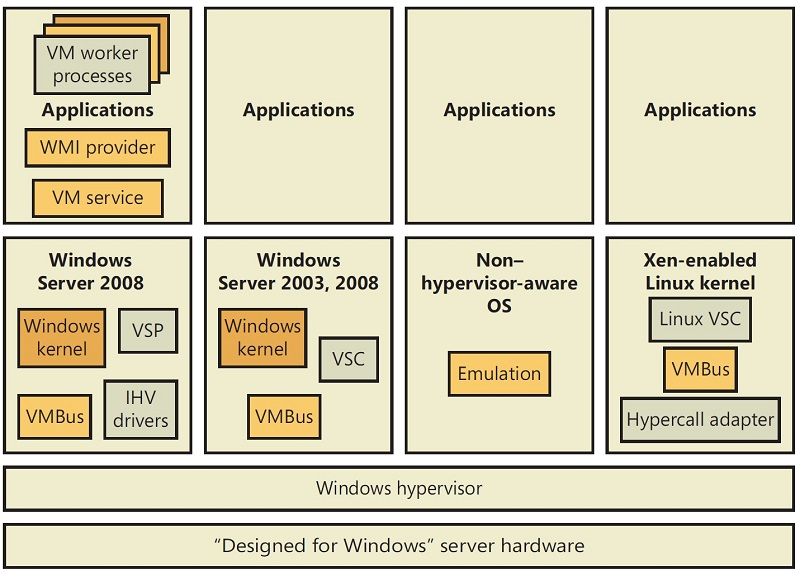
\includegraphics[height=7cm]{fig/hyperv_architektura.jpg}
  \caption{Architektura Hyper-V \cite{WindowsInternalsPart1}}
  \label{fig:hypervarchitektura}
\end{figure}

\paragraph{IIS} 
Internet Information Services je webový server s podporou rozšiřujících modulů. Podporuje protokoly HTTP, HTTPS, FTP, FTPS, SMTP a NNTP. Podporuje různé autentizační metody, např. Windows autentizace a klientský certifikát. Od verze 7.0 IIS má modulární architekturu.  Moduly, neboli rozšíření (extensions), mohou být přidány nebo odstraněny samostatně, nezávisle na sobě.
Existují různé typy modulů k zajištění bezpečnosti, pro správu obsahu, komprese, cachování, logování a diagnostiku. Je dostupné rozšíření Web Deployment Tool, které umožňuje nasazení webových aplikací na IIS server. \cite{MasteringWindowsServer}

\paragraph{Storage Spaces} 
Technologie, která umožňuje virtualizovat úložiště dat pomocí seskupení disků do tzv. storage pools a pak vytvoření virtuálních disků nazývané storage spaces. Podporované možnosti jsou: Simple (bez duplikace), Mirror (zrcadlo s dvěma disky), Parity (distribuovaná parita, 3 disky). \cite{MasteringWindowsServer}

\paragraph{DHCP a DNS Server role} 
Role pro podporu protokolů DHCP a DNS. DHCP se používá pro automatickou konfiguraci počítačů připojených do sítě. DHCP server přiděluje počítačům IP adresu, masku sítě, implicitní bránu a adresu DNS serveru. DNS je hierarchický systém doménových jmen. Jeho hlavním úkolem je převod doménových jmen na IP adresy a naopak. \cite{MasteringWindowsServer}

\paragraph{Windows Update Services (WSUS)} 
WSUS je služba zajišťující aktualizaci softwaru pro operační systém Windows. Je to vlastně lokálně spravovaná podoba služby Windows Update. \cite{MasteringWindowsServer}

\paragraph{Remote Desktop Services (Terminal Services)} 
Pomocí této technologie je možné převzít kontrolu vzdáleného počítače. Na klienty je přenášeno jenom GUI rozhraní. Vstupy uživatele jsou přenášeny zpátky na server, kde jsou zpracovávány. \cite{MasteringWindowsServer}

\paragraph{Windows Deployment Services} 
Umožňuje vzdálené nasazení operačního systému Windows. Funguje na základě technologie PXE (Preboot Executioni Environment). \cite{MasteringWindowsServer}

\paragraph{Windows Remote Management}
WinRM je implementace protokolu WS-Management společnosti Microsoft. Protokol WS-Management je založen na základě protokolu SOAP (Simple Object Access Protocol). WS-Management a WinRM umožňují, aby různé hardwarové a softwarové komponenty vzájemně mezi sebou komunikovali. Na rozdíl od technologie DCOM (Distributed COM), WinRM nevyžaduje složitou konfiguraci firewallu. \cite{MasteringWindowsServer}

\paragraph{PowerShell Desired State Configuration}
PowerShell DSC je nová platforma ve Windows PowerShell. Umožňuje nasazení a správu konfigurace služeb a prostředí. DSC rozšiřuje jazyk Windows PowerShell. Poskytuje nové Windows PowerShell funkce (cmdlety) a zdroje (resources), pomocí kterých je možné deklarativně popsat požadovaný stav a konfigurace. Příklady použití: zapínání/vypínání role a funkce operačního systému, správa registrů, souborů a služeb, nasazení nového software, spouštění Windows PowerShell skriptů a zjištění aktuální konfigurace. \cite{dsc}

\subsection{Microsoft SQL Server}
SQL server je vysoce výkonný relační databázový systém založený na architektuře klient-server. Je škálovatelný, bezpečný a integrovaně pracuje s jazykem XML. 

SQL Server 2014 má tři edice:
\begin{itemize}
\item Enterprise: nejvyšší edice, jsou dostupná všechny funkce
\item Standard: limitované funkce Business Intelligence, typicky vhodné pro malá organizace
\item Business Intelligence: nabízí různé BI schopnosti -- reporting a analytics, Power View a Power Pivot. Vhodné pro organizace, které nepotřebují výkonný a škálovatelný OLTP, dostupný v edici Enterprise.
\end{itemize}

Dále jsou dostupná i jiná speciální edice: Developer, Web a Express.

Mezi hlavními komponenty patří: databázové jádro, reportování, služby pro analýzu a integraci dat, replikace, hlášení, fulltextové vyhledávání a Service Broker.

Nástroje dostupné pro správu: Microsoft SQL Management Studio, SQL Server Configuration Manager (konfigurace síťových protokolů), SQL Server Profiler (zachycování události ze serveru).  \cite{SqlServerIntro}

\subsection{TeamCity}
TeamCity je výkonný nástroj pro podporu kontinuální integrace. Pro správu používá webové rozhraní. Podporuje celou škálou různých prostředí a platforem. Na obrázku \ref{fig:teamcityoverview} je vidět webové rozhraní aplikace\footnote{TeamCity demo je dostupné na adrese \url{https://teamcity.jetbrains.com/overview.html}}. Mezi hlavní výhody patří: 

\begin{itemize}
\item Rozsáhlá podpora různých nástrojů: TeamCity má zabudovanou podporu pro velké množství systémů, např. Visual Studio, MSBuild, MSTest, GitHub, TFS, PowerShell, Bash, atd.
\item Rozsáhlá podpora konfigurace
\item Build History: funkce test history, change log, pinned builds, různé statistiky
\item Rozšiřitelnost: REST API, plugins, Third Party HTML reporty
\item Code Quality tracking: např. zabudovaný Code Coverage
\end{itemize}

Jsou dostupné i jiné nástroje (konkurence TeamCity): Jenkins/Hudson, TFS Build, Bamboo, CruiseControl, GitLab. \cite{TeamCity}

\begin{figure}[]
  \centering
  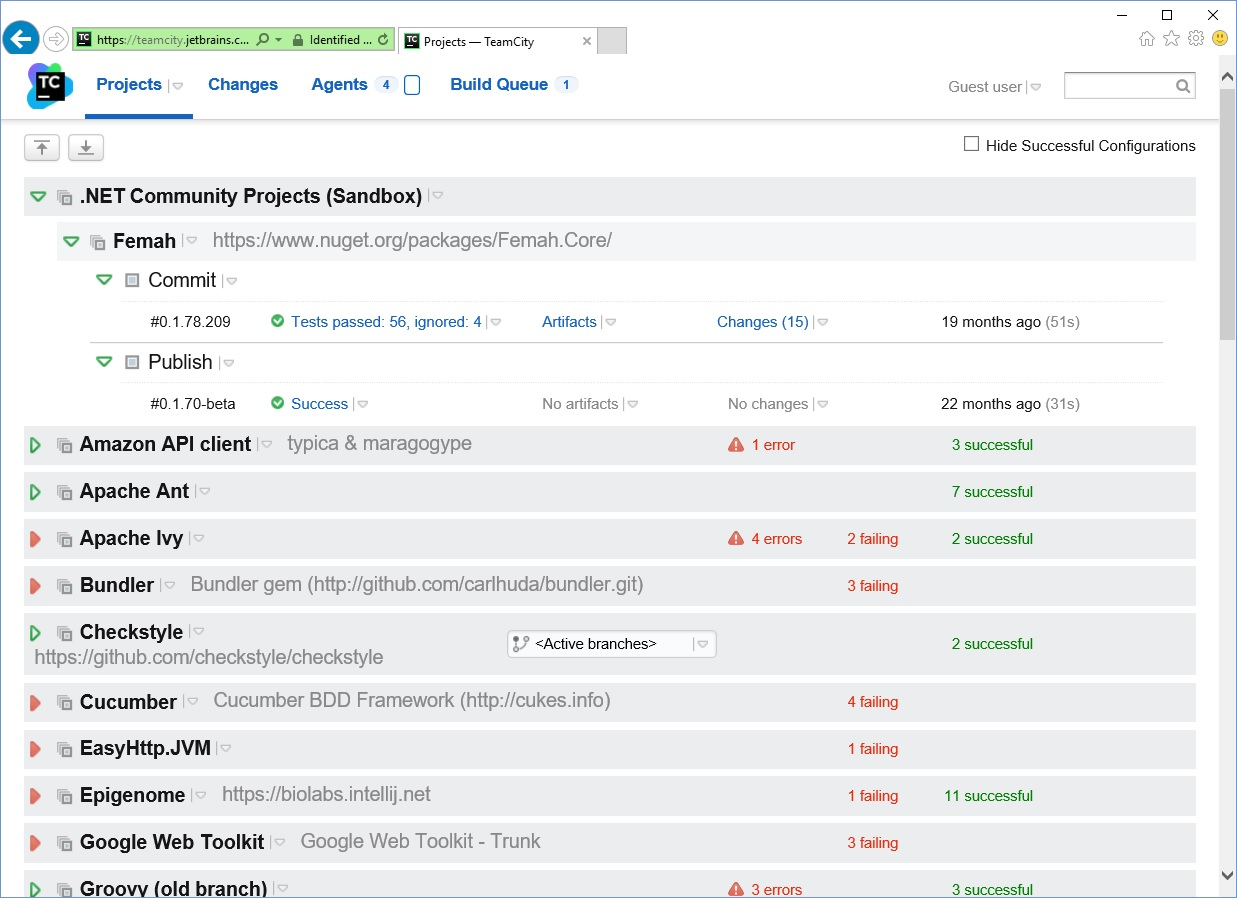
\includegraphics[height=10cm]{fig/teamcity_overview.jpg}
  \caption{Webové rozhraní v TeamCity}
  \label{fig:teamcityoverview}
\end{figure}

\subsection{Chef}
Chef je framework, pomocí kterého je možné jednoduše spravovat infrastrukturu. Chef je založen na skriptovacím jazyce Ruby. Umožňuje spravovat fyzické i virtuální servery. Vytvoříme dokonalé kopie hotových prostředí, bez zádrhelů. Hlavní komponenty je vidět na obrázku \ref{fig:chefoverview}:

\begin{itemize}
\item Server: obsahuje konfigurace pro každý registrovaný uzel
\item Workstation: lokální Chef, tady pracuje vývojář
\item Node (uzel): klient, který je registrovaný na serveru. Má nainstalovaného agenta, který je nazván Chef client.
\item Chef Analytics: platforma, která poskytuje různé akce, historie, real-time reporty a notifikace.
\item Chef Supermarket: open source adresář, kde jsou dostupné cookbooky, které byli vyvinuté komunitou Chef.
\end{itemize}

Pojem \uv{cookbook} patří mezi nejdůležitějšími nástroji Chef. Obsahuje konfigurace (tz. recipe), které musí být provedeny na uzlech. Každý cookbook definuje jeden kompletní scénář. \cite{ChefHandsOnLab}

\begin{figure}[]
  \centering
  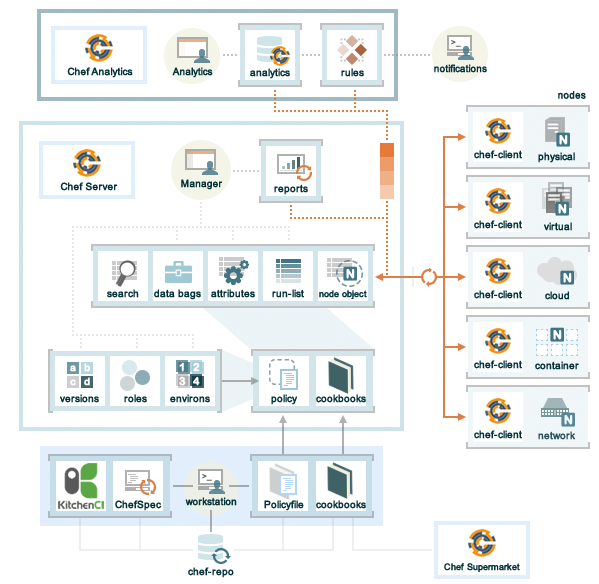
\includegraphics[height=9cm]{fig/chef_overview.png}
  \caption{Přehled Chef}
  \label{fig:chefoverview}
\end{figure}

Konkurence Chefu je Puppet od firmy Puppet Labs. Výborné porovnání těchto nástrojů je dostupné na url \url{http://www.infoworld.com/article/2614204/data-center/puppet-or-chef--the-configuration-management-dilemma.html}. Hlavními výhodami Chefu jsou: jazyk Ruby (Puppet používá vlastní jazyk), zcela open-source bez omezení a podpora TDD (Test Driven Development) pomocí nástroje kitchen.

Obrázek \ref{fig:chefoverview} byl převzat z webové stránky dostupné na \url{https://www.upguard.com/articles/puppet-vs.-chef-revisited}.

\subsection{Nástroje k řízení nasazovacího procesu}
\paragraph{HashiCorp Atlas}
Umožňuje rychlé nasazení pomocí automatizovaného pracovního pos-tupu. Nasazovací proces rozšíří o možnost nastavení různých politik a pravidel. Atlas je velice flexibilní nástroj, ale i přesto poskytuje jednoduché a samoobslužné nasazování. \footnote{viz \url{https://www.hashicorp.com/atlas.html}}

\paragraph{Octopus Deploy}
Octopus Deploy velice dobře spolupracuje s buildovacím serverem, aby umožnil spolehlivé, bezpečné a automatizované nasazení ASP.NET webových aplikací a Windows služeb do testovacích a produkčních prostředí. Podporuje nasazení do kloudu, ale i do lokálních prostředí. \footnote{viz \url{https://octopus.com/}}

\paragraph{ThoughtWorks Go}
ThoughtWorks Go je open source Continuous Delivery server. Umožňuje vytvoření pokročilých deployment pipelinů. Placená podpora a různá rozšíření jsou dostupné taky, aby usnadnili komplikované scénáře. \footnote{viz \url{https://www.thoughtworks.com/go/}}

\paragraph{TFS Release Management}
Tento nástroj je součástí Microsoft TFS serveru. Umožňuje: automatizovat nasazení, odsouhlasení jednotlivých kroků, pokročilé logování, podporu bezpečnostních politik, snadné nasazení do Azure, rozsáhlou podporu rozšíření. \footnote{viz \url{https://www.visualstudio.com/en-us/features/release-management-vs.aspx}}

\paragraph{Chef Delivery}
Produkt od společnosti, která vytvořila i nástroj Chef. Jako ostatní nás-troje, podporuje vytvoření pracovních postupů. Srdcem řešení je vlastně platforma Chef. \footnote{viz \url{https://www.chef.io/delivery}}

\subsection{Jiné technologie}
\paragraph{ASP.NET MVC 5}
ASP.NET MVC je webový aplikační framework, který implementuje vzor MVC (Model-View-Controller). Je to lehký, vysoce testovatelný framework, který je integrovaný s existujícímí funkcemi ASP.NET. \cite{aspnetmvc}

\paragraph{Application Insights}
Služba poskytovaná firmou Microsoft v kloudu Azure. Umožňuje monitorovat a diagnostikovat webové i mobilní aplikace, detekovat problémy a sledovat využití.\footnote{viz \url{https://azure.microsoft.com/en-us/services/application-insights}}

\chapter{Praktická část}
\label{ch:impl}
V této kapitole se budeme zabývat s aplikací poznatků z předchozí kapitoly na naši ukázkovou aplikaci. Začínáme specifikací a návrhem aplikace, následně ukážeme implementaci jednotlivých částí, nástrojů a vytvoření ukázkového prostředí. 

\section{Úvod a specifikace}
Představme si, že pracujeme ve vývojářské firmě a dostali jsme úkol vytvořit aplikaci. Tato aplikace má být webovým informačním systémem, který eviduje peněžní transakce. Slouží jako interní nástroj, pomocí kterého lze analyzovat finanční toky. Důležitým požadavkem je, aby aplikace obsahovala i různé reporty. Některé transakce je potřeba elektronicky podepisovat a je vyžadována integrace s existujícími systémy používanými zákazníkem. Předem jsme stanovili, že budeme stavět na platformě společnosti Microsoft, tzn. .NET Framework a operačním systému Windows. Naše firma má více zákazníku, kteří mají zájem o tento nový produkt. Právě proto je důležité upozornit na skutečnost, že prostředí, do kterého budeme nasazovat, není homogenní.  

Nemáme přístup do všech prostředí a je možné, že různí zákazníci mají různé nároky na konfigurace. Proto nelze aplikovat jednoduchý scénář, ve kterém bychom měli několik stejně nakonfigurovaných serverů a které bychom měli úplně pod kontrolou. Někdy nám zákazník umožní pouze omezený přístup např. k databázovým serverům.

Snažíme se používat agilní metodiky. Klademe veliký důraz na prototypování. Zákazník chce pravidelně vidět aktuální stav vývoje. Má možnost určit směr vývoje, prioritizovat vývoj jednotlivých funkcí a pravidelně kontrolovat, jestli produkt splňuje jeho očekávání. Pro nás nejsou tak důležité konkrétní a podrobné funkce aplikace, spíš to, že daná část aplikace vůbec existuje a má určitou funkci.

Po analýze požadavku jsme identifikovali následující části:
\begin{itemize}
\item webová aplikace: klasická ASP.NET MVC 5 aplikace. Běží na aplikačním serveru IIS, v operačním systému Windows Server.
\item Microsoft SQL databáze: v aplikaci slouží jako úložiště dat.
\item klientské nástroje: prohlížeč neumí pracovat s různými integracemi a elektronickými podpisy, proto je potřeba, aby na klientských stanicích byly dostupné i desktopové aplikace. Komunikace mezi webovou stránkou a aplikací zajistí URI handlery.
\item reporty: Microsoft Reporting Services Report Server
\item scheduler: aplikace, která slouží k provádění pravidelných akcí.
\end{itemize}

Na obrázku \ref{fig:architektura} vidíme základní architekturu aplikace. V následujících kapitolách ukážeme, jak splnit výše uvedené požadavky z hlediska nasazení. Aplikace bude nasaditelná již od začátku. Vycházíme z prázdného projektu a postupně přidáváme nové části. Budeme stavět komponenty, které lze využívat i pro jiné aplikace. Není nutné dodržet přesné pořadí jednotlivých kroků.

\begin{figure}[]
  \centering
  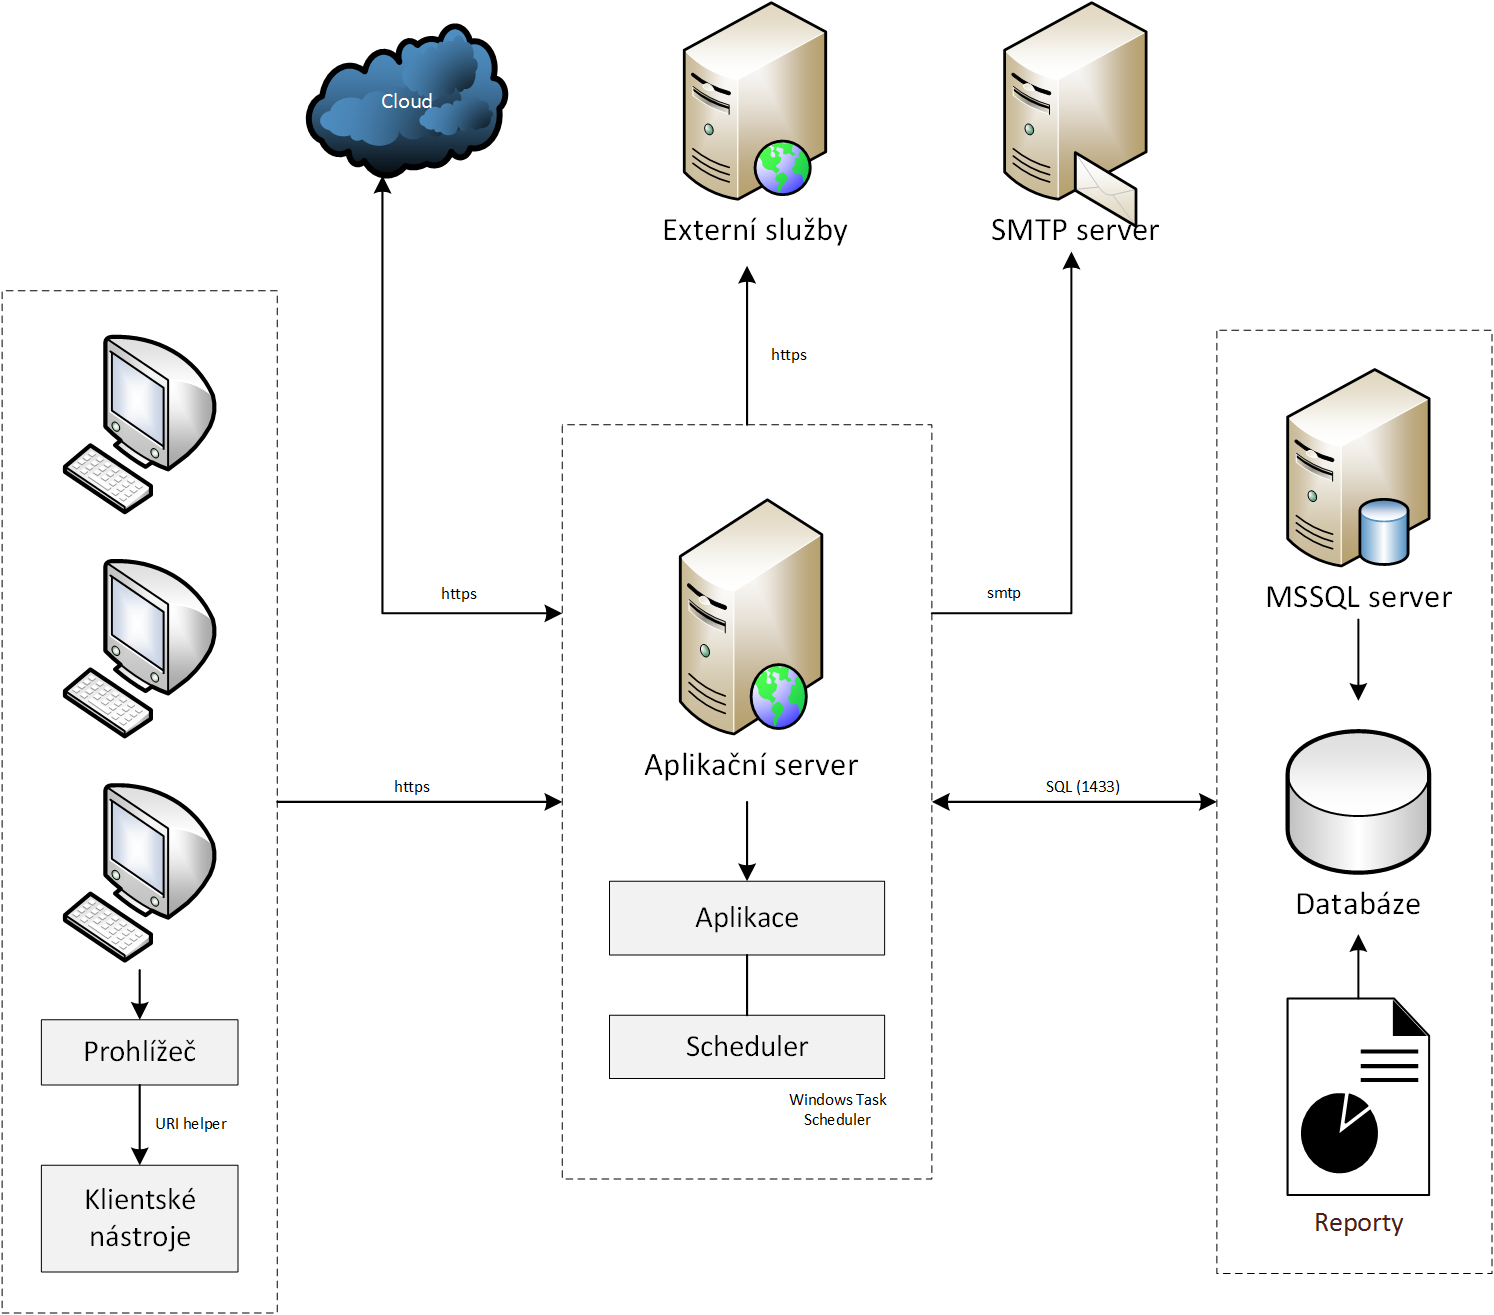
\includegraphics[height=10cm]{fig/app_architektura.png}
  \caption{Architektura ukázkové aplikace}
  \label{fig:architektura}
\end{figure}

\section{Přehled struktury projektu}
Implementace aplikace a nástrojů je rozdělena do dvou částí:

\begin{itemize}
\item projekty Cadmus a Hector: znovupoužitelné knihovny a nástroje
\item projekt Nyx: ukázkový projekt
\end{itemize}

Zdrojové soubory jsou dostupné na přiloženém médiu a taky na stránkách GitHubu\footnote{\url{https://github.com/mdavid626/triton}}. Výstupy z projektu Cadmus jsou publikovány jako NuGet balíčky. NuGet feed je hostován na stránkách MyGet\footnote{\url{https://www.myget.org/feed/Packages/cymric}}. 

Ukázková aplikace se jmenuje Nyx a lze ji nasadit na libovolný Windows Server, který splní určité prerekvizity. Podrobný popis nasazení uvidíme v dalších kapitolách. Vzdálený přístup příkazové řádky k serverům zajistíme pomocí technologie PowerShell Remoting. Konfigurace spravujeme pomocí speciálního editoru konfigurace. 

Virtuální počítače vytvoříme pomocí nástroje Vagrant, boxy sestavíme pomocí Packer. Konfigurace serverů a nainstalování prerekvizit budeme provádět pomocí nástroje Chef. Kontinuální integrace zajistí TeamCity a vydané verze spravuje Visual Studio Team Services (Release manager). Po úspěšném nasazení získáme funkční webovou aplikaci a databáze, jsou nasazeny reporty a aplikace scheduler. Na klientské stanici jsou nainstalovány naše klientské nástroje. 

Struktura projektu ve verzovacím systému je následovní:

\begin{itemize}
\item \texttt{src/Nyx}
\begin{itemize}
\item \texttt{Nyx.ClientTools}: klientské nástroje
\item \texttt{Nyx.ClientTools.Setup}: MSI instalátor klientských nástrojů
\item \texttt{Nyx.Cloud}: kloudové nástroje
\item \texttt{Nyx.Data}: knihovna pro přístup k databázi
\item \texttt{Nyx.DbProject}: databázový projekt
\item \texttt{Nyx.DbUp}: obsahuje migrační skripty
\item \texttt{Nyx.Doc}: obsahuje dokumentace (prázdné)
\item \texttt{Nyx.Environments}: obsahuje konfigurace prostředí
\item \texttt{Nyx.Foundation}: obsahuje základní třídy z projektu Nyx
\item \texttt{Nyx.Reporting}: obsahuje reporty
\item \texttt{Nyx.Scheduler}: aplikace scheduler
\item \texttt{Nyx.Web}: webový projekt
\item \texttt{Nyx.Web.Tests}: jednotkové testy webového projektu
\item \texttt{Nyx.Web.UiTests}: UI testy webové aplikace
\end{itemize}
\item \texttt{src/Tools/Cadmus}
\begin{itemize}
\item \texttt{Cadmus.DbUp}: obsahuje obecnou funkcionalitu k migraci databází
\item \texttt{Cadmus.Foundation}: základní, obecně použitelné třídy
\item \texttt{Cadmus.Foundation.Tests}: jednotkové testy projektu Foundation
\item \texttt{Cadmus.Packer}: skripty a konfigurace sestavení Vagrant boxů
\item \texttt{Cadmus.ParameterEditor}: editor konfigurace
\item \texttt{Cadmus.Parametrizer}: knihovna pro editaci XML konfigurace
\item \texttt{Cadmus.Protector}: podpora šifrování pomocí DPAPI
\item \texttt{Cadmus.Scripts}: obsahuje PowerShell moduly a různé skripty
\item \texttt{Cadmus.VisualFoundation}: základní, obecně použitelné třídy pro WPF aplikaci
\end{itemize}
\item \texttt{src/Tools/Hector}: obsahuje projekt pro naši Visual Studio extension
\end{itemize}

\section{Implementace webové aplikace}

\subsection{Webová aplikace}
Webové aplikace ASP.NET lze nasadit různými způsoby. Nejjednodušším z nich je pouhé kopírování souboru do určité složky na aplikačním serveru. Takový postup má však svoje problémy. Neumí totiž upravit parametry webu (např. soubor \texttt{web.config}), ani aktualizovat nebo vytvořit webovou aplikaci v IIS. 

Další možností je využít nástroj Web Deploy. Tento nástroj je dostupný jako rozšíření do serveru IIS. Konfigurace spočívá ve vytvoření profilu nasazení, který je pak umístěn ve složce \texttt{<Projekt>/Properties/PublishProfiles}. Používá formát XML a je to vlastně MSBuild skript. Vytvoření (sestavení) balíčku lze pak zajistit pomocí příkazu:

\texttt{msbuild <solution.sln> /p:DeployOnBuild=true /p:PublishProfile=Deploy}

Výstupem je rovněž několik souborů: \texttt{Nyx.deploy.cmd}, \texttt{Nyx.SetParameters.xml},\\ \texttt{Nyx.SourceManifest.xml} a \texttt{Nyx.zip}. XML soubory slouží ke konfiguraci parametrů webu, \texttt{deploy.cmd} skript ke spuštění instalace a \texttt{Nyx.zip} obsahuje soubory webu.

Další parametry webu, jako např. konfigurace aplikačního poolu, vytvoření Web Site-ů, lze udělat pomocí nástroje \texttt{appcmd}, který je standardně součástí instalace IIS. Existuje i lepší způsob, a to použití PowerShell. Nejdříve je potřeba naimportovat příslušný modul: \texttt{PS> Import-Module WebAdministration} a pak použít dostupné funkce \texttt{New-WebAppPool}, \texttt{New-Website} a pod.

Většina dnešních webových aplikací již běží nad protokolem HTTPS. Certifikát naimportujeme pomocí PowerShell funkce (\texttt{Import-Certificate}). Další krok je navázání certifikátu na port 443. To lze zajistit pomocí příkazu \texttt{netsh http add sslcert}. Naše ukázková aplikace běží nad protokolem HTTP, takže konfiguraci certifikátu nebudeme provádět.

Byl vytvořen PowerShell modul \texttt{Cadmus.Web.psm1}, který obsahuje následující důležité funkce:
\begin{itemize}
\item \texttt{Deploy-WebApp}: nasadí webovou aplikaci
\item \texttt{Deploy-WebSite}: vytvoří Web Site a aplikační pool
\item \texttt{Start-WebMaintenance}: nastartuje maintenance mód, vypíná webovou aplikaci
\item \texttt{Stop-WebMaintenance}: vypíná maintenance mód
\end{itemize}

Modul dále obsahuje funkci \texttt{Parametrize-SetParametersFile}, která nakonfigurované parametry propaguje do potřebných souborů.

Ke zjednodušení nasazení webové části aplikace může náš nasazovací tým, ale i vývojáři, využívat tento již hotový PowerShell modul. Konfigurace  musí předat jako argumenty, zatím neexistuje žádné centrální úložiště konfigurace prostředí.

\begin{figure}[]
  \centering
  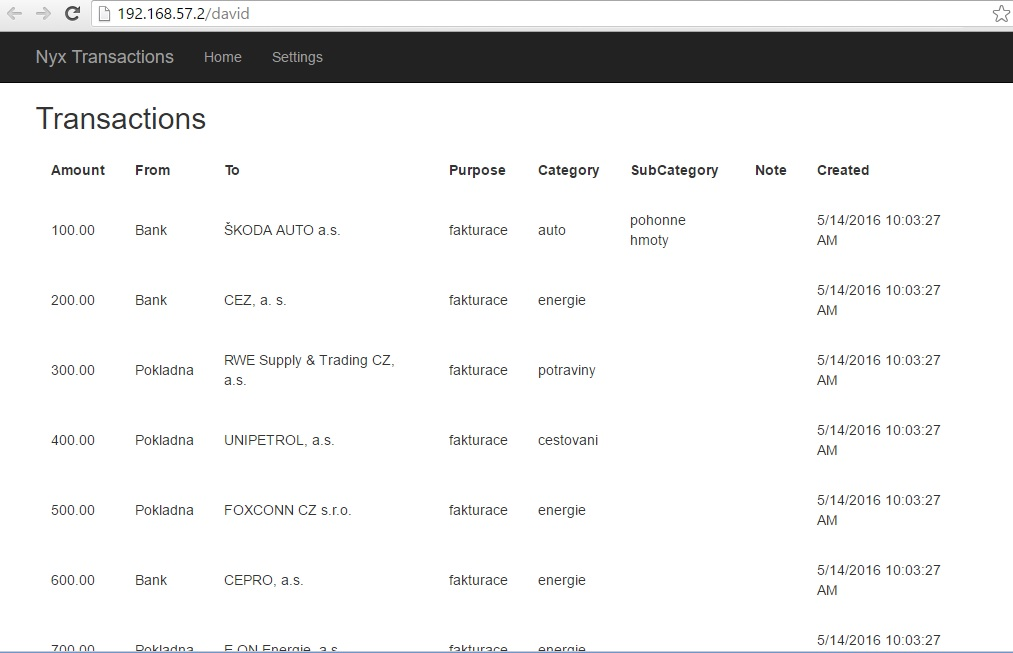
\includegraphics[width=15cm]{fig/web.jpg}
  \caption{Webová stránka ukázkové aplikace}
  \label{fig:web}
\end{figure}

\subsection{Verzování schémat relační databáze}
Zásady kontinuální integrace musíme aplikovat nejen na zdrojový kód aplikace, ale i na databázi. Znamená to, že je potřeba: 

\begin{itemize}
\item verzovat databázové objekty: tabulky, triggery, procedury, funkce atd.
\item vytvořit mechanizmus, pomocí kterého lze automatizovaně tyto objekty aktualizovat během nasazování. 
\end{itemize}

Nejdřív zajistíme ukládání verze databáze do jednoduché tabulky \texttt{SchemaVersions}. Tabulka se skládá ze tří sloupců: \texttt{Id}, \texttt{ScriptName} a \texttt{Applied}. Tato tabulka bude evidovat informace o aplikovaných verzí.

Verzování schémat databáze ve Visual Studio lze provést pomocí databázového projektu. V našem případě je to projekt \texttt{Nyx.DbProject}. Aktualizační mechanizmus, tzn. mechanizmus k povýšení verze databáze, obsahuje projekt \texttt{Nyx.DbUp}. 

Úprava databázového schématu vypadá následovně:

\begin{enumerate}
\item V databázi provedeme libovolné změny.
\item Pomocí nástroje Schema Comparision (Tools $\rightarrow$ SQL Server $\rightarrow$ New Schema Comparision) provedeme porovnání databázového projektu a databáze.
\item Změny promítneme do databázového projektu.
\item Pomocí Schema Comparision lze nechat vygenerovat změnový SQL skript. Pokud potřebujeme, není problém tento skript napsat zcela ručně.
\item Vytvořený změnový skript zaverzujeme do projektu \texttt{DbUp}. Existuje složka \texttt{Scripts}, která obsahuje tyto skripty. Soubory jsou přímo vložené do výsledného exe souboru, proto musíme nastavit atribut \texttt{Build Action} na \texttt{Embedded Resource}.
\item Verze databáze zapíšeme i do souboru v databázovém projektu.
\end{enumerate}

Povýšení databáze pak provedeme spuštěním programu \texttt{DbUp} z příkazové řádky: \texttt{DbUp.exe /upgrade}

Jak vidíme, projekt \texttt{Nyx.DbUp} obsahuje jenom databázové skripty. Funkcionalitu obsahuje projekt \texttt{Cadmus.DbUp}, který slouží jako znovupoužitelný prvek. Vychází z knihovny \texttt{DbUp} (dostupná na \url{nuget.org} jako NuGet balíček). Provedlo se několik úprav a doplnili se různé parametry příkazové řádky, kontroly a logování. DbUp umí navíc vytvořit novou databázi pomocí dacpac balíčku a argumentem \texttt{/drop} lze odstranit již nepotřebnou databázi. 

Uvedený postup vytvoření verze databáze obsahuje mnoho manuálních kroků, tzn. je náchylný k chybám. Abychom proces zjednodušili a předešli chybám, bylo vytvořeno rozšíření do Visual Studia (Hector). Toto rozšíření umí nastavit atribut změnových skriptů \texttt{Build Action} na \texttt{Embedded Resource}, založit prázdné skripty a zapsat verze. Continuos Delivery nám říká, že máme zjednodušit a automatizovat proces nasazení. Patří do toho i tyto záležitosti. 

Migrace a databázové operace v procesu nasazení řídí PowerShell modul\\ \texttt{Cadmus.Database.psm1}. Nejdůležitějšími funkcemi z modulu jsou: \texttt{Create-Database},\\ \texttt{Migrate-Database}, \texttt{Setup-DbUserAccount}. Tento modul umí i jakési jednoduché parametrizace SQL skriptů. Funguje to na základě proměnných, které jsou ve formátu: \texttt{\$(název)}.

Náš tým již má nástroje, které umožní jednoduše povýšit schéma databáze. Skripty jsou tvořeny vývojáři během vývoje a ne před, nebo během nasazení.

\subsection{Klientské nástroje}
Naše klientské nástroje jsou vlastně jednoduché .NET aplikace. Tady se budeme zabývat s tím, jak tyto aplikace dostat na klientské stanice. Jednoduchým řešením je použít klasický MSI (Microsoft Installer) instalátor. Takový instalátor ve Visual Studiu dokážeme vytvořit mnoha způsoby. My jsme se rozhodli pro nástroj WiX Toolset. Jde o projekt \texttt{Nyx.ClientTools.Setup}. Je potřeba soubory aplikace nakopírovat,  pak ještě nastavit URI handler v registrech. Hlavním konfiguračním souborem je \texttt{Produkt.wsx}.

Balíčky MSI lze nainstalovat z příkazové řádky pomocí nástroje \texttt{msiexec}. Příklad použití: \texttt{msiexec /i /qn Nyx.ClientTools.Setup.msi}, kde \texttt{/i} znamená instalace, \texttt{/qn} zajistí, aby nebylo zobrazeno žádné uživatelské rozhraní. Administrátor může provádět instalace např. pomocí Group Policy. Tento přístup má ale tu nevýhodu, že je potřeba, aby počítače byly v doméně a instalace byla provedena až po restartování počítače.

Jako alternativu budeme používat možnost instalace pomocí PowerShell Remoting. Nejdřív instalátor nakopírujeme na klientské stanice (\texttt{Copy-Item}), pak instalaci spustíme pomocí \texttt{Invoke-Command} a \texttt{msiexec}. Povolení a konfigurace PowerShell Remotingu uvidíme v následujících kapitolách. Funkcionalitu obsahuje modul \texttt{Cadmus.Msi.psm1}, který má jednu funkci \texttt{Deploy-Msi}. Jedna nevýhoda je, že klientské stanice musí být zapnuty během nasazení.

\subsection{Testování}
Není naším cílem podrobně popsat různé testovací metody, jako např. jednotkové testy, integrační testy atd., nicméně se ale do určité míry musíme zmínit o testování. Naše automatizované metody vyžadují, aby jejich výstupy bylo možné automatizovaně otestovat. 

Většina dnešních vývojářů je již zvyklých na použití jednotkových testů. Dalším mohou být testy uživatelského rozhraní, které lze vytvořit pomocí nástroje Selenium.

Důležité je skripty a nástroje konfigurace infrastruktury otestovat. Lze to zajistit např. pomocí nástroje \texttt{kitchen}, který je součástí Chef Development Kitu, přičemž testování spouštíme příkazem \texttt{kitchen converge}. 

\subsection{Reporty}
Naše ukázková aplikace obsahuje i reporty, které byly vytvořeny pro Microsoft SQL Server Reporting Services server. Balíček reportů se skládá z několik souborů:
\begin{itemize}
\item .rdl: soubory popisující vzhled a obsah jednotlivých reportů
\item .rds: obsahují informace o přístupu do databáze (Shared Data Source)
\item .rptproj: projektový soubor, eviduje reporty a ostatní soubory
\end{itemize}

Nasazovat reporty na Report Server lze provádět mnoha způsoby. Nejjednodušším způsobem je nástroj příkazové řádky \texttt{rs.exe}, který spouští Visual Basic skripty k provedení nasazení reportů. My ale budeme využívat přímo HTTP služby poskytnuté report serverem. Proxy třídu vytvoří skript \texttt{New-SSRSWebServiceProxy.ps1} a samotné nasazení provede skript \texttt{Deploy-SSRSProject.ps1}. Tyto skripty byly převzaty z webu \url{https://gist.github.com/ChrisMissal/5979564}. 

Funkcionalitu obalí PowerShell modul \texttt{Cadmus.Report.psm1}. Obsahuje funkce \texttt{Deploy-Report} a \texttt{Parametrize-DataSourceFile}. 

V rámci nasazení jsou vytvořeny složky, jsou nasazeny datové zdroje a samotné reporty. Konfigurace přístupových práv pro uživatele nejsou součástí nasazení. Parametrizace datového zdroje podporuje jenom Integrated Security. 

Nasazovací tým může využít tento nový modul. K nahrání reportů již nemusí používat webové rozhraní, všechny reporty jsou nahrány pomocí jednoho příkazu.

\subsection{Scheduler}
Mnoho webových aplikací potřebuje pravidelně spouštět různé úkoly. K těmto účelům slouží aplikace Scheduler. Tento nástroj obsahuje několik úloh, které spouští opakovaně dle konfigurace. Konfigurace je uložena v databázi a je vidět ve webové aplikaci, na stránce Settings. 

Scheduler je nástroj příkazové řádky. Nejdůležitějšími argumenty jsou \texttt{/schedule} a \texttt{/shutdown}. Prvním nastartujeme plánované úlohy a druhý slouží k vypnutí aplikace scheduler. Jednotlivé úlohy mohou běžet dlouho, proto musí existovat mechanizmus, jak požádat scheduler o vypnutí. Konfigurace úloh je v databázové tabulce \texttt{SchedulerItem}. Každá úloha pak implementuje rozhraní \texttt{ITask}, které má jednu metodu \texttt{Execute}. Jednotlivé úlohy jsou spouštěny asynchronně. 

Samotný scheduler pravidelně vzbudí Windows Task Scheduler. Proto je potřeba vytvořit během nasazení záznam do Windows Task Scheduleru. Je to vlastně nástroj, velice podobný nástroju \texttt{cron}, známý z platforem Linux a Unix. Záznam vytvoříme pomocí \texttt{schtasks.exe}. Musíme se zmínit o tom, že záznam obsahuje i přihlašovací údaje, pod kterými běží naplánovaná úloha. Tyto údaje musíme dostat bezpečně na náš aplikační server.

Vypnutí aplikace scheduler funguje následovně: 

\begin{itemize}
\item Je povolena pouze jedna instance aplikace provádějící spouštění plánovaných úloh. To je zajištěna pomocí tzn. mutexů. Název mutex-u se skládá z identifikátoru databáze a názvu aplikace. Identifikátor databáze je unikátní GUID, které je uloženo v tabulce \texttt{DatabaseInfo}.
\item Po spuštění aplikace vytvoří komunikační kanál, ve kterém bude naslouchat různé žádosti. Tento kanál je vytvořen pomocí tzn. named pipes. Jeden z podporovaných žádostí je žádost vypnutí. Po obdržení žádosti scheduler nastaví CancellationToken a tím požádá běžící úlohy o vypnutí. Úlohy dle vlastního uvážení mohou reagovat na žádost a své činnosti ukončit. 
\end{itemize}

Příslušný PowerShell modul je \texttt{Cadmus.Scheduler.psm1}. Nasazovaní provádí funkce \texttt{Deploy-Scheduler}. Vypnutí, tzv. maintenance mód spustí funkce \texttt{Start-SchedulerMaintenance}.

\subsection{Maintenance mód}
Během nasazení musíme zajistit vypnutí aplikace scheduler a webové aplikace. Nechceme totiž, aby uživatelé pracovali s naší aplikací, která může být v nekonzistentním stavu.

Vypnutí webové aplikace lze zajistit pomocí souboru \texttt{appoffline.htm}, který nakopírujeme do kořenové složky webové aplikace. Tento speciální soubor zná IIS a jakmile ho uvidí, webovou aplikaci okamžitě vypne a vrátí obsah tohoto souboru pro každou žádost. Obsah webové stránky během nasazení vidíme na obrázku \ref{fig:maintenance_mode}.

Pozornější čtenáři si určitě všimli, že maintenance mód nemáme pro naše reporty a klientské nástroje. Zajistit vypnutí reportů není nijak jednoduché, Report Server takovou funkcionalitu vůbec nemá. Mohli bychom naše reporty skrýt, ale rozhodli jsme se problematiku neřešit. Reporty slouží v podstatě jenom ke čtení dat a proto se nemusíme obávat, že se databáze dostane do nekonzistentního stavu.

\begin{figure}[]
  \centering
  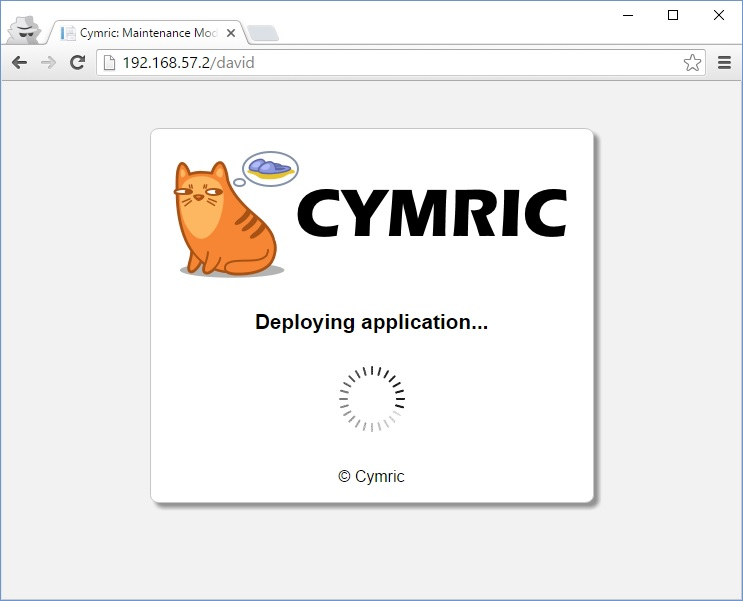
\includegraphics[height=7cm]{fig/maintenance_mode.jpg}
  \caption{Maintenance mód webové aplikace}
  \label{fig:maintenance_mode}
\end{figure}

\subsection{Blue/Green nasazení}
Blue/Green nasazení znamená, že aplikaci nasadíme do dvou identických prostředí, ze kterých je živý vždy pouze jeden. V případě, že nasazení selže, jednoduše přepneme zpátky na to funkční prostředí. Znamená to ale dvojnásobné nároky na hardware. 

Nejjednodušším, avšak neúplným postupem je, provozovat a nasazovat pouze jednu webovou aplikaci, ale mít dvě fyzické složky. Přepínání pak lze zajistit úpravou parametru PhysicalPath -- aplikace ukazuje na první nebo druhou složku. Bohužel tento postup neřeší např. různé nastavení webové aplikace, aplikačního poolu nebo Web Sity. Dále existuje možnost nasadit dvě různé webové aplikace, ale do jedné, společné Web Sity. Přepínání je možné pomocí parametru VirtualPath: jeden parametr bude nastaven na požadovanou adresu a ten druhý s postfixem test nebo podobně. 

Opravdové Blue/Green je možné implementovat pomocí tzn. load balanceru, který žádosti routuje buď na Blue nebo na Green server. Je potřeba ale duplikovat úplně všechno: aplikační a databázové servery, reporty, scheduler atd.

Implementovat Blue/Green nasazení je velice náročné na zdroje, proto tento postup v této práci aplikovat nebudeme. Pro představu uvedeme postup, jak bychom mohli postupovat:

\begin{itemize}
\item Nainstalovat a nakonfigurovat load balancer: např. Nginx nebo podobný produkt. Samozřejmě můžeme mít i dedikovaný fyzický stroj.
\item Zjistíme aktuálně živé prostředí a zapneme pro toto prostředí maintenance mód (tzn. web zcela vypneme nebo přepneme do read-only módu)
\item Uděláme kopii živé databáze do druhého prostředí.
\item Nasadíme aplikace do druhého prostředí.
\item Provedeme různé kontroly a testy a když nasazení vyhovuje, požádáme load balancera, aby žádosti již routoval na naše druhé prostředí.
\item Pokud nasazení nevyhovuje, stačí jednoduše vypnout maintenance mód na živém prostředí.
\end{itemize}

Spolehlivost nasazení naší ukázkové aplikaci zajistíme bez Blue/Green a to následovně:

\begin{itemize}
\item nasazení jsou rychlá a automatizovaná
\item před migrací provedeme zálohování databáze
\item aplikace scheduler je vypnuta před nasazením
\item instalátory předchozí verze aplikace jsou přístupné 
\item konfigurace a nasazení je zcela automatizované
\item konfigurace a nasazení je často a automaticky testováno
\end{itemize}

\subsection{Kontinuální integrace}
\label{ch:ciserver}
K zajištění kontinuální integrace budeme používat TeamCity. Webové rozhraní je vidět na obrázku \ref{fig:cymric_teamcity}. Struktura projektů je následovná:
\begin{itemize}
\item Nyx: projekt pro ukázkovou aplikaci
\begin{itemize}
\item Build: slouží k sestavení aplikace, obsahuje i jednotkové testy
\item AutoDeploy: je spouštěn automaticky po úspěšném sestavení, aplikace nasadí do prostředí Dev/Domino dle konfigurace \texttt{autotest.xml}
\item Deploy: na požádání nasadí aplikace do vybraného prostředí (tzn. self-deployment). Vhodné pro testeři a vývojáře. Vybrat prostředí je možné z předem definovaného seznamu.
\item Publish: publikuje NuGet balíček na MyGet server
\end{itemize}
\item Cadmus: Build a Publish -- sestavení a publikace NuGet balíčku
\item Hector: Build a Publish -- sestavení a publikace VSIX rozšíření
\end{itemize}

\begin{figure}[]
  \centering
  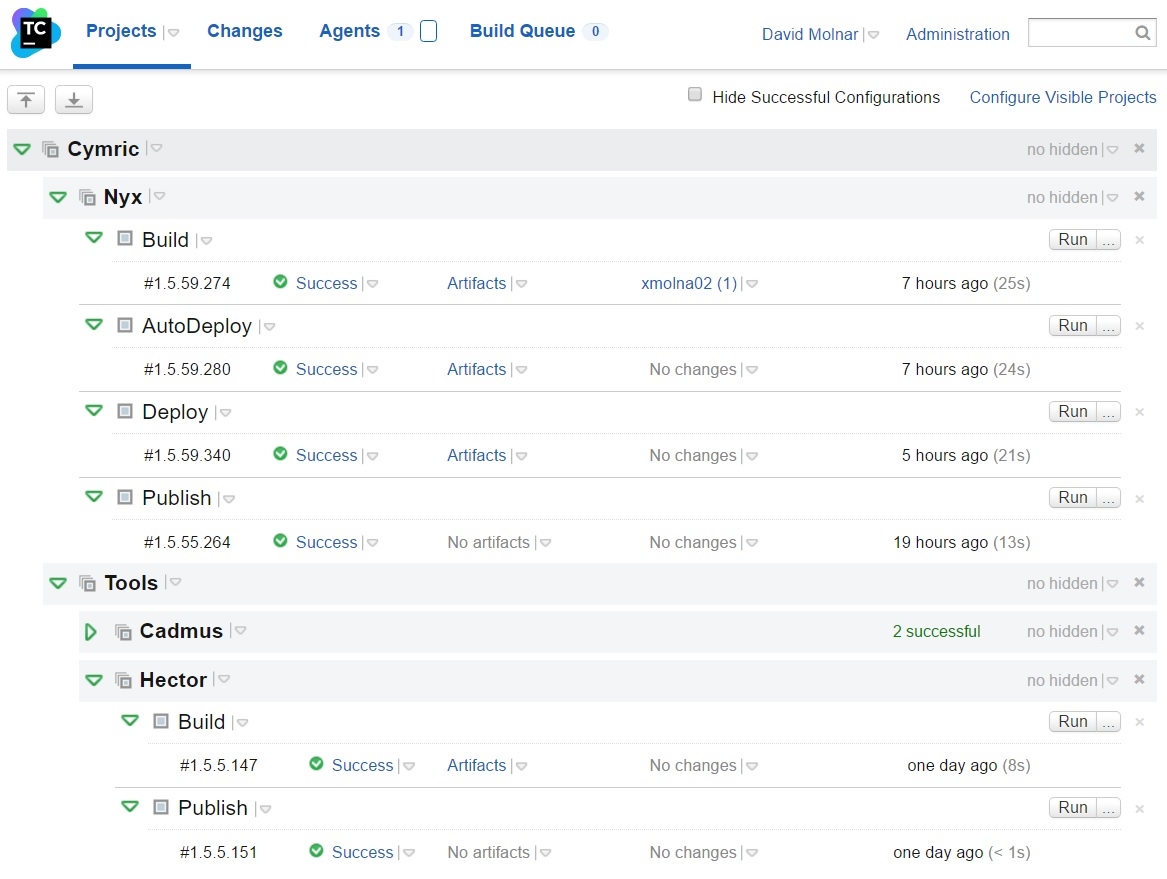
\includegraphics[width=15cm]{fig/teamcity.jpg}
  \caption{Projekty v TeamCity}
  \label{fig:cymric_teamcity}
\end{figure}

\section{Správa infrastruktury}

\subsection{Editor konfigurace}
Tato aplikace je velice důležitá v celém pracovním postupu. Slouží k nastavení konfiguračních parametrů prostředí a aplikace. Parametry můžeme nastavit přímo v konfiguračních souborech,
nicméně klasické textové editory nám v tom nijak nepomůžu. Právě proto vznikl tento editor, který dokáže pomoct s vyplňováním parametrů. Má různé pomocné funkce, které určitě uvítá každý člen nasazovacího týmu (jako např. nápověda, generování AES šifrovacích klíčů pro webové aplikace a editor připojovacích řetězců databází).

Skládá se z několika částá: nahoře je menu a panel nástrojů. V centrální části vidíme parametry, které můžeme editovat. Vedle nich nahoře můžeme vybrat sekce. Každá sekce pak má určité dostupné akce. V dolní části se nachází barevní konzola s výstupy (viz obrázek \ref{fig:nyx_installer}).

Metadata parametrů a dostupných akcí jsou uloženy v XML souboru \texttt{base.xml}. Každý parametr obsahuje titulek, typ editoru, popis a hodnotu. Navíc je podporováno hierarchické skládání konfiguračních souborů, tzn. nakonfigurované parametry můžeme rozložit do více souborů a takto sdělovat konfigurace mezi více prostředími. Příklad použití je vidět v konfiguraci prostředí Dev/Domino (\texttt{src/Nyx/Nyx.Environments/Dev/Domino}): prostředí \texttt{david.xml} a \texttt{marketa.xml} odkazují na \texttt{nyx.xml}, který obsahuje sdílené konfigurace pro obě prostředí.

\begin{figure}[]
  \centering
  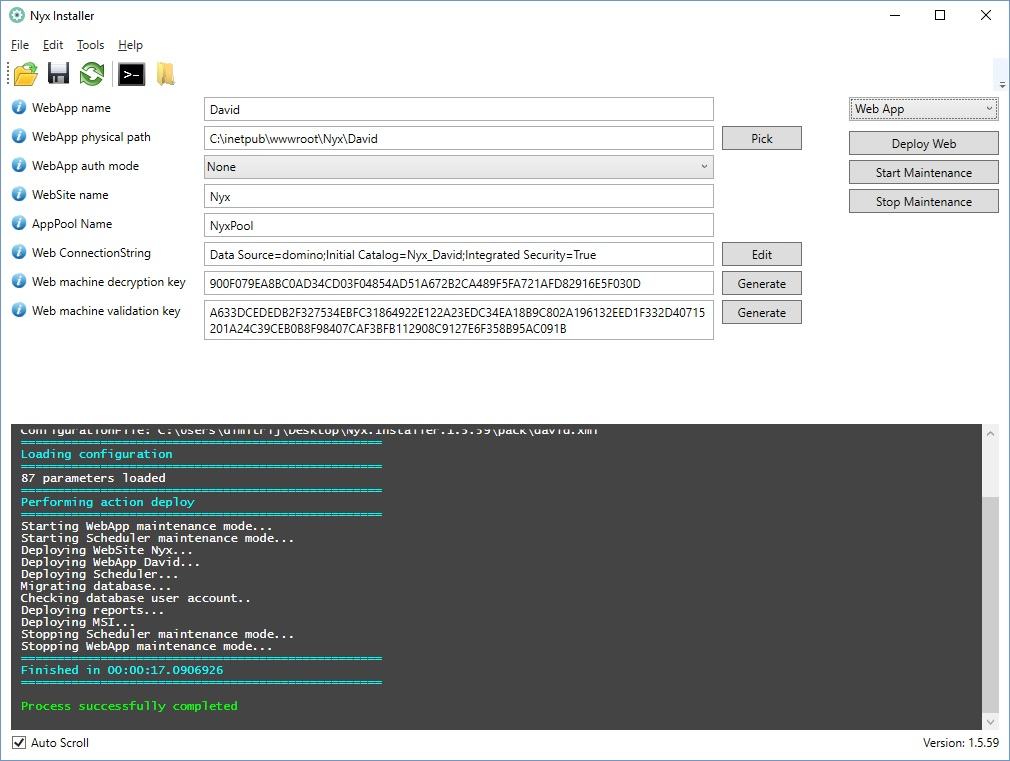
\includegraphics[width=14cm]{fig/installer.jpg}
  \caption{Editor konfigurace}
  \label{fig:nyx_installer}
\end{figure}

Tato aplikace umožňuje, aby nasazovací tým mohl jednotně vytvářet konfigurace jednotlivých prostředí a následně konfigurace uložit do verzovacího systému. Naše PowerShell moduly využívají tyto soubory k získávání potřebné konfigurace. Není tedy potřeba skripty spustit s různými argumenty a je umožněno verzování konfigurace.

\subsection{Šifrování citlivých dat}
Součástí konfigurace prostředí a aplikace jsou i citlivé informace, např. hesla nebo přístupové klíče, které je potřeba zabezpečit. Na tyto účely  byl vytvořen nástroj Protector.

Samozřejmě nám nebude stačit jednosměrné hashování, ale bude potřeba zašifrované data i dešifrovat. Z toho vyplývá, že bude potřeba vyřešit distribuce a správu šifrovacích klíčů. Abychom předešli tomuto problému, budeme používat šifrování zabudované přímo do operačního systému, tzv. DPAPI. O dešifrovacích klíčích se stará operační systém. 

Vznikl tedy nástroj, který vstupní řetězec zašifruje pomocí DPAPI a výsledek vrátí ve formátu BASE64. Grafické rozhraní aplikace vidíme na obrázku \ref{fig:protector}. Editor konfigurace má šifrování zabudované přímo v aplikaci. 

\begin{figure}[]
  \centering
  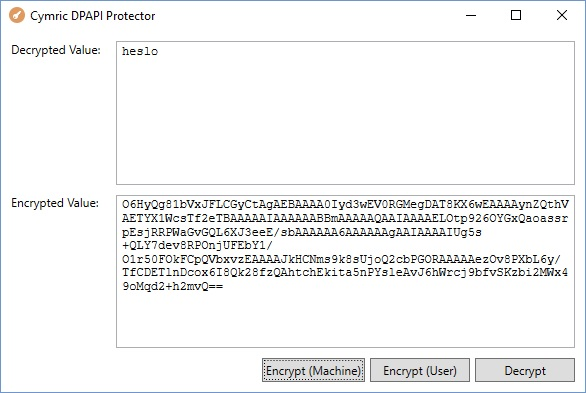
\includegraphics[height=7cm]{fig/protector.jpg}
  \caption{Nástroj Protector}
  \label{fig:protector}
\end{figure}

Příklad použití: víme, že k nastavení aplikačního poolu budeme potřebovat uživatelské jméno a heslo. Tyto údaje chceme uložit do XML konfigurace ve verzovacím systému. Na daném aplikačním serveru spustíme nástroj Protector a heslo zašifrujeme. Výsledek pak zadáme do editoru konfigurace. Hesla dokáže dešifrovat jenom aplikační server. Není tedy žádný problém konfiguraci uložit do verzovacího systému.

\subsection{Vytvoření virtuálních stanic}
Mezi zásady CD patří automatizované vytvoření infrastruktury. Znamená to vytvoření a instalaci serverů a klientských stanic. Samozřejmě fyzický server nelze vytvořit pomocí skriptů, ale virtualizovaný již ano. 

Instalace operačního systému Windows není nijak složité, ale jak již víme, instalaci není vhodné provádět ručně. Naštěstí existuje možnost tzv. bezobslužné (unattended) instalace. Instalátoru poskytneme speciální XML soubor, ve kterém jsou informace, potřebné pro instalátora k dokončení instalace.

Dalším krokem je automatizovat vytvoření virtuálního prostředí. To lze zajistit pomocí nástroje Vagrant. Vagrant má jeden vstupní soubor s názvem vagrantfile, který popisuje, jaké virtuální počítače chceme vytvořit. Obsahuje i konfiguraci, jako např. konfigurace sítě nebo název počítače. Vagrant pracuje s pojmem box, který je jakýsi kontejnerem již hotových, nainstalovaných virtuálních počítačů. 

Vytvoření takových boxů pro operační systém Windows provedeme pomocí nástroje Packer. Tento nástroj spustí bezobslužnou instalaci Windows a výsledek vyexportuje jako Vagrant box. Tuto akci můžeme považovat jako sestavení (build) šablonů virtuálních počítačů.

Jakmile máme vytvořeny boxy, můžeme je naimportovat pomocí příkazu \texttt{vagrant box add "test.box" --name "test"}. Vytvoření a spuštění virtuálního počítače provedeme pomocí příkazu \texttt{vagrant up}. 

V našem případě budeme používat Packer šablony převzaty z \url{http://github.com/mitchellh/packer}. Tyto šablony jsou uloženy v projektu \texttt{Cadmus.Packer}. Bylo provedeno několik úprav, jako např. nastavení časového pásma. Musíme na tomto místě upozornit, že sestavení boxu může trvat velice dlouho. 

V ukázkovém prostředí budeme používat boxy windows\_2012\_r2, windows\_2012\_r2\_sysprep a windows\_10. Konfigurace pro naši ukázkovou aplikaci jsou uloženy v projektu Nyx.Environments. Používaný virtualizační nástroj je Oracle VirtualBox.

\subsection{Konfigurace operačního systému}
\label{ch:serverconfig}
K zajištění instalace prerekvizit a správné konfigurace serverů a klientských stanic budeme používat nástroj Chef. Byl vytvořen jeden tzv. cookbook (cadmus) a 3 skripty (tz. recipes): \texttt{web.rb}, \texttt{sql.rb} a \texttt{client.rb}. První skript, \texttt{web.rb}, konfiguruje aplikační server. Zajistí, aby bylo nainstalováno Web Deploy rozšíření do IIS, .NET Framework 4.5 a potřebné Windows featury (WebServer, Asp.NET 4.5). Umí vytvořit i uživatele a zařadit ho do role IIS\_IUSRS.

Druhý skript, \texttt{sql.rb}, konfiguruje Microsoft SQL server. Nejdříve zajistí instalaci .NET Framework 3.5, která je prerekvizitou instalace SQL serveru. Pak následuje instalace SQL Serveru a otevření SQL portu ve firewallu.  

Třetí skript, \texttt{client.rb}, slouží ke konfiguraci klientských stanic, které mají jedinou prerekvizitu: nainstalovaný .NET Framework 4.5.

Používáme i cookbooky třetí strany, sql-server, dotnetframework, windows a chef\_handler.

Chef konfigurace aplikujeme pomocí PowerShell modulu \texttt{Cadmus.Chef.psm1}. Tento modul dokáže kontrolovat dostupnost Chef klienta, v případě nedostupnosti klient taky nainstalovat. Odkazy na instalátory lze nastavit v editoru konfigurace (viz sekce Provisioning).

\subsection{Nasazovací skripty}
Samotné nasazení spustíme pomocí skriptu \texttt{Deploy.ps1}. Tento skript naimportuje potřebné PowerShell moduly (\texttt{Modules/Cadmus.*.psm1}), načítá konfigurační soubor a spustí nasazení.

Zpracování chyb v PowerShell skriptech je umožněno pomocí výjimek. Pokud chceme reagovat na chyby aplikace příkazové řádky, stačí kontrolovat proměnné \texttt{\$LastExitCode} a následně s příkazem \texttt{throw "chyba!"} vyvolat výjimku.

Je podporováno pokročilé logování. Základem je rozhraní \texttt{ILogger} z \texttt{Cadmus.Foundation}. Jsou dostupné logovací třídy, které logují do souboru a do konzolu. Je možné použít speciální řídicí sekvence, a to např. \{Success\} nebo \{Verbose\}. Výstupy označené verbose jsou logovány jenom do souborů.

Ke komunikaci se vzdálenými servery používáme technologii PowerShell Remoting. Ve výchozím nastavení používá Remoting port 5986. V rámci jedné Windows domény funguje autentizace v Remoting bez další konfigurace. Pokud se ale přihlašujeme do jiné domény (cross-domain), tak buď používáme HTTPS protokol (vyžaduje konfiguraci certifikátu), nebo adresu vzdáleného počítače explicitně povolíme v konfiguraci TrustedHosts. Povolení  automaticky provede editor konfigurace.

\subsection{Release Management}
Jak jsme se o tom již zmiňovali v první kapitole, naši aplikaci chceme nasazovat do různých nehomogenních prostředí. Máme více zákazníků a potřebujeme evidovat a sledovat nasazené verze. Rozhodli jsme se využít online službu Visual Studio Team Services\footnote{viz \url{https://www.visualstudio.com/en-us/products/visual-studio-team-services-vs.aspx}}. Tato služba zahrnuje i jiné produkty, jako verzovací systém a projekt management.

V sekci Releases je vytvořen nový projekt, nazvaný Nyx a několik prostředí. Přehled je vidět na obrázku \ref{fig:releaseman_overview} a \ref{fig:releaseman_releases}. Po vytvoření nového releasu je možné spustit nasazování. Samotné nasazování provede agent, který běží na serveru v našem virtualizovaném prostředí. Agent stahuje instalátor přímo z NuGet feedu, konfiguraci prostředí pak z verzovacího systému.

Jako výsledek získáme informace o tom, kde a jaká verze aplikace je nasazená, kdo a kdy nasazení provedl. Služba podporuje i nastavování přístupových práv a oprávnění. Před nasazením je vyžadováno odsouhlasení. Je to ideální nástroj k nasazení do produkčního prostředí.

\begin{figure}[]
  \centering
  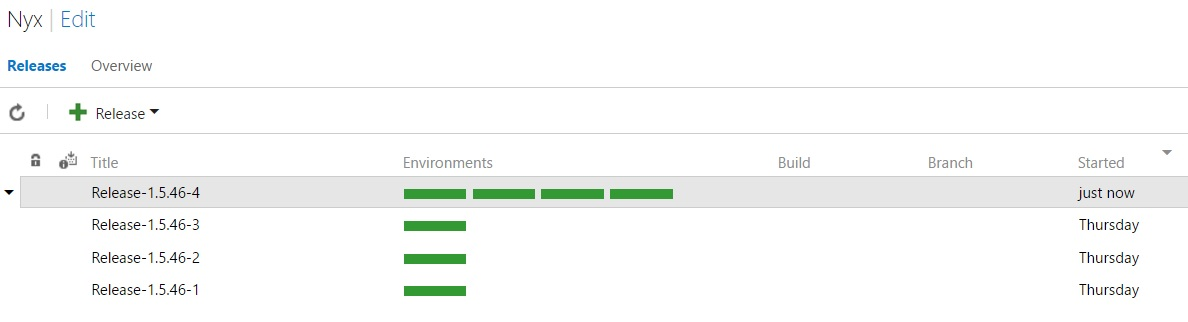
\includegraphics[width=15cm]{fig/releaseman_releases.jpg}
  \caption{Visual Studio Team Services Releases}
  \label{fig:releaseman_releases}
\end{figure}

\begin{figure}[]
  \centering
  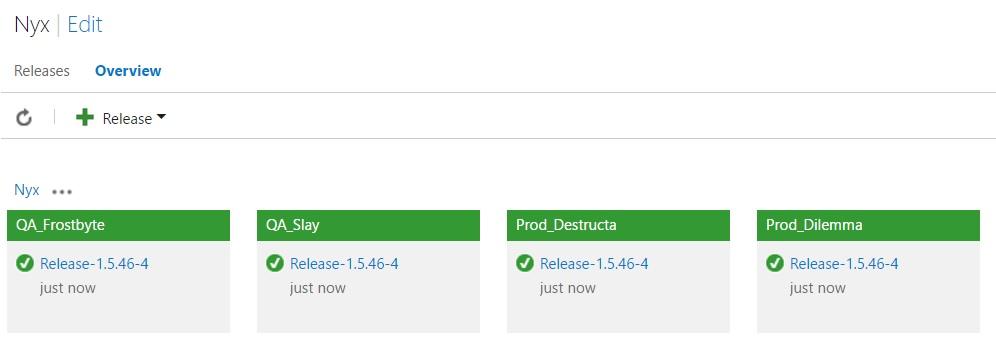
\includegraphics[width=15cm]{fig/releaseman_overview.jpg}
  \caption{Přehled Visual Studio Team Services Release}
  \label{fig:releaseman_overview}
\end{figure}

\section{Ukázkové prostředí}

\subsection{Přehled}
Konfigurace našeho ukázkového prostředí se nachází v projektu \texttt{Nyx.Environments}. Je členěn na tři části: Dev, QA a Prod:
\begin{itemize}
\item Dev: jsou tady dvě prostředí. První, Luna, slouží k lokálnímu testování s jednou webovou aplikací, s názvem Dev. Druhé prostředí, Domino, má více webů, David a Markéta. 
\item QA: testovací prostředí se skládá z 4 počítačů, které jsou v doméně: Active Directory server, aplikační server, SQL server a jedna klientská stanice. 
\item Prod: produkční prostředí, je totožný s QA.
\end{itemize} 

Všechny tyto servery běží virtualizovaně v Oracle VirtualBox. Každé prostředí má svoji vlastní interní síť. 

\subsection{Jak pracovat s ukázkovým prostředím?}
K rozjetí ukázkového prostředí budeme potřebovat nainstalovat prerekvizity. Všechny postupy byly testovány na operačním systému Windows 10 Professional, verze 1511 s nainstalovanými aktualizacemi. Nemělo by být problém použít jiný operační systém, např. Windows 7 nebo Windows 8.1, nicméně tyto systémy nebyly otestovány.

Budeme potřebovat následující software:
\begin{itemize}
\item Oracle VirtualBox 5.0
\item Windows Management Framework 5.0
\item Vagrant
\item .NET Framework 4.6.1
\end{itemize}

Licenční podmínky bohužel nedovolí volnou distribuci těchto softwaru, proto instalátory nejsou uloženy na přiloženém médiu. Sesbírali jsme ale patřiční linky a uložili je na stránce: \url{http://mdavid626.github.io/triton}.

Dále budeme potřebovat Vagrant boxy. Není problém tyto boxy vygenerovat/sestavit pomocí nástroje Packer. Potřebné konfigurace jsou uloženy v projektu \texttt{Cadmus.Packer}. Byly použity konfigurace windows\_2012\_r2 a windows\_2012\_r2\_sysprep. Musíme čtenáře upozornit, že sestavení může trvat hodně dlouho a to hlavně z důvodu instalace aktualizací (až několik hodin). Hotové boxy jsou dostupné ke stažení na adrese \url{http://mdavid626.github.io/triton}. Po stažení naimportujeme boxy pomocí příkazu: \texttt{vagrant box add windows\_2012\_r2\_sql.box --name windows\_2012\_r2\_sql}. Seznam nainstalovaných boxů lze zobrazit pomocí příkazu \texttt{vagrant box list}.

Použité uživatelské účty jsou Administrator (heslo Vagrant123) a vagrant (heslo vagrant).

Jsou dostupné i videa, které demonstrují nasazení ukázkové aplikace. Videa jsou uloženy na přiloženém médiu v složce resources/demo.

\chapter{Vyhodnocení výsledků}
\label{ch:vyslekdy}
V této kapitole vyhodnotíme přínos zásad CD. Porovnáme vývoj, nasazení a údržbu aplikace před a po aplikace CD.

\section{Ruční nasazení}
Představme si, že naše ukázková aplikace je již hotová, ale nasazení provádíme zcela ručně. Nemáme konfigurační soubory, žádné skripty, jenom popis postupu nasazení. Abychom si to lépe představili a dokázali porovnat, uvedeme kompletní postup nasazení. 

Postup nasazení je následovné:

\begin{enumerate}
\item Vytvořit virtuální počítač v Oracle VirtualBox: nakonfigurovat CPU, RAM a síťové připojení. Připojit ISO instalátor operačního systému.
\item Nainstalovat operační systém.
\item Nakonfigurovat název počítače, IP adresu, povolit Remote Desktop.
\item Aplikační server: nainstalovat Windows featury: IIS web server a ASP.NET 4.5. Dále nainstalovat .NET Framework 4.5 a Web Deploy. Instalátory kopírujeme pomocí Remote Desktop nebo získáme ze sdílené složky.
\item Vytvoříme uživatele pro naši aplikaci, nastavíme heslo a přiřadíme ho do skupiny IIS\_IUSRS.
\item SQL Server: nainstalujeme .NET Framework 3.5. Budeme potřebovat soubory ze instalačního média, přesněji složku sources.
\item Nainstalujeme SQL server, můžeme používat grafický instalátor. Zvolíme port a název instance.
\item Konfigurace IIS: odstraníme Default Web Site.
\item Vytvoříme nový aplikační pool. Nastavíme účet a heslo.
\item Vytvoříme nový Web Site, nastavíme aplikační pool a bindings. 
\item Vytvoříme složku, kde budou umístěny soubory aplikace.
\item Na tuto složku nastavíme přístupová práva pro uživatele aplikačního poolu.
\item Vytvoříme webovou aplikaci. Nastavíme aplikační pool, fyzickou cestu a název Web Sity. 
\item Nakopírujeme soubory webové aplikace. 
\item Konfigurace SQL: vytvoříme novou databázi. 
\item Pro účet aplikačního poolu nastavíme přístup do SQL serveru a k databázi.
\item Spustíme skript k vytvoření struktur v databázi. Aktuální skript připraví databázový specialista před nasazením. Pokud databáze již existuje, spustíme migrační skripty.
\item Otevřeme port 1433 k zajištění komunikace s aplikačním serverem.
\item Scheduler: vytvoříme složku a nakopírujeme soubory aplikace Scheduleru.
\item Musíme taky nastavit přístupová práva na tuto složku.
\item Vytvoříme Task ve Windows Task Scheduleru, nakonfigurujeme účet, triggery a akce.
\item Nasadíme reporty: vytvoříme složky na report serveru. Přes webové rozhraní nahrajeme rdl a rds soubory.
\item Nainstalujeme klientské nástroje.
\item Konfigurace webové aplikace, scheduleru a reportů: nastavíme přístup do databáze. Ve webové aplikaci dále nastavíme typ autentizace na None, vygenerujeme a nastavíme nové AES šifrovací klíče. 
\item Výsledek otestujeme.
\end{enumerate}

Aktualizace aplikace je samozřejmě jednodušší, ve většině případů stačí aktualizovat soubory webové aplikace. Vývoj aplikace je rychlý, prerekvizity se mění často a dynamicky. Co to pro nás znamená? Hlavně to, že při každém nasazení je potřeba prerekvizity a konfigurace aplikace konzultovat s vývojáři nebo číst a analyzovat dokumentaci. 

Dalším velkým problémem je, že konfigurační parametry nejsou nikde uloženy, jedině na provozním serveru. Pokud potřebujeme vytvořit velice podobné, nebo identické prostředí, tak celý postup musíme opakovat. Pokud v organizaci pracuje víc administrátorů, není zcela jasné, kdo a co přesně nakonfiguroval. Pokud tedy něco nefunguje, je velice problematické a náročné hledat chyby.

Vydat novou verzi aplikace tým nedělá příliš často, protože nasazovací proces je velice komplikovaný a hlavně časově náročný. Z toho ale přímo vyplývá, že každé nasazení obsahuje obrovské množství změn. Vývojář nemá možnost jak jednoduše otestovat změny v aplikaci. Jednak nechápe nasazovací proces a ani na to nemá čas -- proces je složitý a časově náročný. 

Vývojový tým neví, která verze kde je nasazená. Sice dokáže to nějak zjistit, ale tyto informace nejsou rychlo dostupné. 

Nasazování často končí chybou: nefungující migrační skript, chybí různé neznámé prerekvizity (typicky nějaká knihovna) nebo kvůli nesprávné konfigurace.

\section{Nasazení pomocí CD}
Náš tým se rozhodl zavést nasazení pomocí CD. Začalo automatizovat nasazení:

\begin{enumerate}
\item Vytvořili Web Deploy balíček k nasazení webu. Balíček je zatím importován ručně z konzolu IIS Manager.
\item Vytvořili nástroj DbUp a databázový projekt. Migrační skripty jsou vytvořeny během vývoje a jsou testovány ihned.
\item Abychom práci zjednodušili a předešli chybám, vývojáři vytvořili rozšíření do Visual Studia, pomocí kterého je možné rychle a automatizovaně vytvořit migrační skripty a záznamy v databázovém projektu.
\item Dalším krokem je vytvoření základní verze editoru konfigurace a základního konfiguračního souboru.
\item Tým vytvoří jednoduchý skript, který dokáže vytvořit webovou aplikaci a naimportovat Web Deploy balíček z příkazového řádku. Skripty parametrizuje a spouští z editoru konfigurace.
\item Nasazovací tým vytvoří základní konfiguraci již existujících prostředí a soubory zaverzuje.
\item Mezi nasazovacími skripty je přidán skript k nasazení scheduleru. Editor konfigurace a parametry jsou taky rozšířeny.
\item Dalším rozšířením je přidání instalátoru klientských nástrojů.
\item Instalátor je průběžně testován. Server kontinuální integrace s každou změnou nasadí novou verzi aplikace do testovacího prostředí.
\item Tým přidá maintenance mód, nasazování reportů a možnost šifrování.
\item V této chvíli je možné použít instalátor v produkčním prostředí.
\item Nasazovací tým vytvoří potřebné konfigurace a nakonfiguruje Visual Studio Team Services Release manager.
\item Jsou vytvořeny konfigurace pro nástroj Vagrant a sestaveny Windows boxy.
\end{enumerate}

Jak vidíme, aktualizace aplikace je mnohem jednodušší. Existuje testovatelný pracovní postup, jak aplikaci nasadit. Nové prerekvizity a konfigurace neznamená žádný problém pro tým, vývojáři a administrátoři rozšíří nebo upraví patřičné soubory a výsledek bez problémů otestuje. Problémy jsou identifikovány včas, opravy lze jednoduše naplánovat a realizovat. Nasazení již neznamená stres a napětí, protože nasazování před použitím v produkčním prostředí je důkladně a automatizovaně otestováno. Nasazovací tým provede nesprávnou konfiguraci již méně často. 

Nové verze aplikace jsou vydávány mnohem častěji. Každá verze obsahuje málo změn. Z toho vyplývá, že případné problémy je možné odstranit v krátkém čase. Každý člen týmu vidí, kde a jaká verze aplikace je nasazena. Určité rozhodnutí pak může udělat na základě těchto informací. 

\chapter{Závěr}
\label{ch:zaver}
Zavést Continuous Delivery kompletně není jednoduché. Celý vývojový tým se musí naučit myslet jinak. Je to časově velice náročný proces. Jakmile ale vyřešíme ty nejnáročnější problémy, získáme potřebné znalosti a dovednosti, můžeme si užívat výhody, které nám poskytuje CD. Nasazení již nebudou těžké a problematické, stresující situace pro vývojový tým, ale jejich každodenní aktivita. 

Zpočátku byl operační systém Windows navržen s grafickým rozhraním. Administrace a konfigurace systémů a různých software-ů byla ve většině případů možná pomocí grafického rozhraní. Dnes je situace naštěstí mnohem lepší, existují nástroje jako PowerShell, PowerShell Remoting a jiné, které nám práci usnadní do významné míry. 

V této práci se nám podařilo vytvořit kompletní pracovní postup. Začínáme vytvořením virtuálních stanic pomocí nástroje Vagrant. Po vytvoření konfigurace provedeme instalaci prerekvizit pomocí Chef skriptů. Následuje nasazení samotné aplikace: vytvoříme aplikační pool, WebSitu, webovou aplikaci, nasadíme scheduler, reporty a nakonec klientské nástroje. Každou část je možné spustit i samostatně. Celý postup byl navržen tak, aby bylo možné vynechat libovolné části a aby se umožnili i ruční zásahy. K umožnění vzdáleného přístupu používáme technologie PowerShell Remoting. Vyřešili jsme i situace, kdy během nasazení potřebujeme citlivé informace, a to šifrováním pomocí služby operačního systému DPAPI.

Mezi nevýhody CD patří, že pořádná implementace vyžaduje hodně času. Vytvořit a udržovat konfigurační skripty není jednoduché. Automatizace na začátku může být nepříjemnou záležitostí. Nicméně i přesto se vyplatí investovat do toho čas a úsilí, protože dokáže významně zjednodušit a zefektivnit dodání softwarových produktů.

%=========================================================================
